%%%%%%%%%%%%%%%%%%%%%%%%%%%%%%%%%%%%%%%%%
\documentclass[a5paper,doc,10pt,noapacite]{apa6}
%----------------------------------------------------------------------------------------
%	Paquetes y configuraciones
%----------------------------------------------------------------------------------------
\usepackage[hidelinks]{hyperref}
\usepackage[unnumberedbib,notocbib]{apacite}
%\usepackage{chapterbib} % bibunits???
\usepackage{bibunits}

\usepackage{amsfonts} 
\usepackage{amsmath}
\usepackage{amssymb,amsthm}
\usepackage{enumerate}
\usepackage{enumitem}
\usepackage[utf8]{inputenc}
\usepackage[T1]{fontenc}
\usepackage[spanish,es-nolayout,es-nodecimaldot,es-tabla]{babel}
\geometry{top=2.5cm, bottom=2.5cm, left=2.5cm, right=2.5cm, headheight=1.8cm,headsep=.5cm,footskip=1.3cm}

\usepackage{url}
\def\UrlBreaks{\do\/\do-}
\def\pnorm||#1||_#2,#3{||#1||_{L^{#2}(#3)}}
\usepackage{multirow}
\usepackage{multicol}
\usepackage{enumitem}
\usepackage{nicefrac}
\usepackage{graphicx}
\usepackage{stmaryrd}
\usepackage{dsfont}
\usepackage{bropd}
\usepackage{easybmat}
\usepackage[table,xcdraw]{xcolor}
\usepackage{longtable} 
\usepackage{setspace}
\usepackage{comment}
\usepackage{mathpazo}
\usepackage{array}
\usepackage{wrapfig}
\usepackage{ragged2e}
\usepackage{hyperref}
\usepackage{bigstrut}
\usepackage{tabularx}

\usepackage{sectsty}
\sectionfont{\centering\fontsize{13}{15}\selectfont}

\subsectionfont{\centering\fontsize{10}{10}\selectfont\scshape}
\subsectionfont{\fontsize{9.5}{10}\selectfont}

\subsubsectionfont{\centering\fontsize{9}{10}\selectfont}
\paragraphfont{\centering\fontsize{8.5}{10}\selectfont}

\usepackage[titles]{tocloft}
\usepackage{textcomp }

\usepackage{csquotes}
\usepackage{floatrow}

\newfloatcommand{capbtabbox}{table}[][\FBwidth]

% Comandos
\newcommand{\bull}{\textbullet \ }
\newcommand{\EPN}{Escuela Politécnica Nacional}
\newcommand{\Modemat}{Centro de Modelización Matemática, ModeMat-EPN}%{ModeMat -- Escuela Politécnica Nacional}
\newcommand{\Modematb}{Centro de Modelización Matemática, ModeMat-EPN}

\newcommand{\R}{\mathbb{R}}
\newcommand{\N}{\mathbb{N}}
\newcommand{\Z}{\mathbb{Z}}
\newcommand{\C}{\mathbb{C}}
\newcommand{\dsum}{\displaystyle \sum}
\newcommand{\yds}{\qquad\text{y}\qquad}
\newcommand{\tendsto}[1][ ]{\stackrel{ #1 }{\longrightarrow}}
\newcommand{\subKeps}[2][k]{#2_{#1,\varepsilon}}
\DeclareMathOperator{\Dom}{Dom}
\DeclareMathOperator{\Ran}{Ran}
\DeclareMathOperator{\inv}{inv}
\DeclareMathOperator{\Res}{Res}
\DeclareMathOperator{\Ind}{Ind}
\DeclareMathOperator{\im}{Im}
\DeclareMathOperator{\CEiP}{CEiP}
\DeclareMathOperator{\dive}{div}
\DeclareMathOperator{\Esp}{E}
\DeclareMathOperator{\Var}{V}
\DeclareMathOperator{\cov}{cov}
\DeclareMathOperator{\Normal}{\mathcal{N}}
\DeclareMathOperator{\sen}{sen}

\newtheorem{definicion}{Definición}
\newtheorem{proposicion}{Proposición}
\newtheorem{teorema}{Teorema}
\newtheorem{observ}{Observación}
\newtheorem{ejem}{Ejemplo}
\newtheorem*{objetivo}{Objetivo}
\newtheorem*{objetivos}{Objetivos}


%%%mycolors
\definecolor{palegreen}{rgb}{0.6, 0.98, 0.6}
\definecolor{paleblue}{rgb}{0.69, 0.93, 0.93}
\definecolor{pastelyellow}{rgb}{0.99, 0.99, 0.59}
\definecolor{pastelgray}{rgb}{0.81, 0.81, 0.77}
\definecolor{pastelgreen}{rgb}{0.47, 0.87, 0.47}
\definecolor{pastelblue}{rgb}{0.68, 0.78, 0.81}

\newcommand{\vsb}{\vspace{0.75\baselineskip}}
\newcommand{\Speaker}[4]{\vsb #1 \\ \emph{#2} \\ \textsc{#3}\\ \texttt{#4}}


\setlength{\parindent}{0pt}
\linespread{1.5}

\usepackage[10pt]{moresize}

\usepackage{xspace}
\makeatletter
\DeclareRobustCommand{\maybefakesc}[1]{%
  \ifnum\pdfstrcmp{\f@series}{\bfdefault}=\z@
    {\fontsize{\dimexpr0.8\dimexpr\f@size pt\relax}{0}\selectfont\uppercase{#1}}%
  \else
    \textsc{#1}%
  \fi
}
\newcommand\AM{\,\maybefakesc{am}\xspace}
\newcommand\PM{\,\maybefakesc{pm}\xspace}
\makeatother


%---------------------------------------- Autoría ---------------------------------------- %
\title{Plantilla LAWOC}
\author{Andy}
\shorttitle{}
\date{\today}

%---------------------------------------- Citas  ------------------------------------------ %
\renewcommand\bibliographytypesize{\footnotesize}


%------------------------------------- Abstracts ---------------------------------------- %
\newcommand{\pto}{$\cdot$ }

% AbstractA no contiene elementos bibliográficos
\newcommand{\AbstractA}[6]{%
	\addcontentsline{toc}{subsection}{#1 \footnotesize(\emph{#2})}
	\begin{center}
		\bf\scshape#1
	\end{center}
	%\subsection{#1}
	\vspace{-0.85\baselineskip}
	%
	%
	\begin{center}
		{\scriptsize% 
			  #2		\bull			% Autor
		\textsf{#3}		\bull			% Institución
		\texttt{#4}		\\[-1em]		% Correo
		\emph{#5} }				%.Área
	\end{center}
	\vspace{-0.5\baselineskip}
	\begin{spacing}{1.2}
		\footnotesize
		\hspace{15.0pt}
		#6	
	\end{spacing}
	\vspace{1\baselineskip}
}

% AbstractCA no contiene elementos bibliográficos
\newcommand{\AbstractCA}[7]{%
	\addcontentsline{toc}{subsection}{#1 \footnotesize(\emph{#2})}
	\begin{center}
		\bf\scshape#1
	\end{center}
	%\subsection{#1}
	\vspace{-0.85\baselineskip}
	%
	%
	\begin{center}
		{\scriptsize% 
			  #2					% Autor
			  #3		\bull			% Co-autores
		\textsf{#4}		\bull			% Institución
		\texttt{#5}		\\[-1em]		% Correo
		\emph{#6} }				%.Área
	\end{center}
	\vspace{-0.5\baselineskip}
	\begin{spacing}{1.2}
		\footnotesize
		\hspace{15.0pt}
		#7	
	\end{spacing}
	\vspace{1\baselineskip}
}

% Abstract B sí contiene bibliografía
\newcommand{\AbstractB}[6]{%
	\addcontentsline{toc}{subsection}{#1 \footnotesize(\emph{#2})}
	\begin{center}
		\bf\scshape#1
	\end{center}
	%\subsection{#1}
	\vspace{-0.85\baselineskip}
	%
	\begin{center}
		{\scriptsize% 
			  #2		\bull			% Autor
		\textsf{#3}		\bull			% Institución
		\texttt{#4}		\\[-1em]		% Correo
		\emph{#5} }				%.Área
	\end{center}
	\vspace{-0.5\baselineskip}
	\begin{spacing}{1.2}
		\begin{bibunit}
			\footnotesize
			\hspace{15.0pt}
			#6
			\addtocontents{toc}{\protect\setcounter{tocdepth}{-1}}	
			\putbib
			\addtocontents{toc}{\protect\setcounter{tocdepth}{2}}
		\end{bibunit}\vspace{0.5\baselineskip}
	\end{spacing}
}

% Abstract B sí contiene bibliografía
\newcommand{\AbstractCB}[7]{%
	\addcontentsline{toc}{subsection}{#1 \footnotesize(\emph{#2})}
	\begin{center}
		\bf\scshape#1
	\end{center}
	%\subsection{#1}
	\vspace{-0.85\baselineskip}
	%
	\begin{center}
		{\scriptsize% 
			  #2					% Autor
			  #3		\bull			% Co-autores
		\textsf{#4}		\bull			% Institución
		\texttt{#5}		\\[-1em]		% Correo
		\emph{#6} }				%.Área
	\end{center}
	\vspace{-0.5\baselineskip}
	\begin{spacing}{1.2}
		\begin{bibunit}
			\footnotesize
			\hspace{15.0pt}
			#7
			\addtocontents{toc}{\protect\setcounter{tocdepth}{-1}}	
			\putbib
			\addtocontents{toc}{\protect\setcounter{tocdepth}{2}}
		\end{bibunit}\vspace{0.5\baselineskip}
	\end{spacing}
}

% Curso tutorial
\newcommand{\Tutorial}[5]{%
\addcontentsline{toc}{section}{#1 \footnotesize(\emph{#2})}
	\begin{center}
		\bf\scshape #1
	\end{center}
	%\subsection{#1}
	\vspace{-0.85\baselineskip}
	%
	\begin{center}
		{\scriptsize% 
			  #2		\bull			% Autor
		\textsf{#3}		\bull			% Institución
		\texttt{#4}		\\[-1em]		% Correo 
		}
	\end{center}
	\vspace{-0.5\baselineskip}
	%
	
	\begin{spacing}{1}
		\begin{bibunit}
			\footnotesize
			#5
			%\addtocontents{toc}{\protect\setcounter{tocdepth}{0}}	
			\putbib
%			\addtocontents{toc}{\protect\setcounter{tocdepth}{1}}
		\end{bibunit}\vspace{0.5\baselineskip}
	\end{spacing}
}

%------------------------------------- Información turística ---------------------------------------- %

\newcommand{\InfoTour}[6]{%
\qquad \textbf{\textsc{#1:}}%
#2

\qquad
\begin{tabular}{p{1.5cm} p{7cm}}
	Hours 	& #3
	\\
	Location	& #4
	\\
	Prices	& #5
    \\
    Website & {\scriptsize\texttt{#6}}
\end{tabular}
\vspace{\baselineskip}
}

\newcommand{\InfoTourb}[2]{%
\qquad \textbf{\textsc{#1:}}%
#2
\vspace{\baselineskip}
}

\newcommand{\InfoTourc}[6]{%
\quad \emph{#1:}%
#2

\quad
\begin{tabular}{p{1.5cm} p{7cm}}
	Hours 	& #3
	\\
	Location	& #4
	\\
	Prices	& #5
    \\
    Website & {\scriptsize\texttt{#6}}
\end{tabular}
\vspace{\baselineskip}
}

\newcommand{\Rest}[3]{%
\begin{tabular}{>{\bf\scshape}p{3.5cm} >{\em\centering\arraybackslash}p{2cm}    >
{\raggedleft\arraybackslash}p{4cm}}
	#1  & #2 & #3
\end{tabular}
\vspace{0.4\baselineskip}
}

\renewcommand{\BCBT}{}

% -------------- Pseudo definición fuera de entorno que no me gustó pero toca respetar las malas costumbres de algún modo

\newcommand{\neodefi}[1]{%
	\vspace{1\baselineskip}
	\textbf{\small#1} \newline
}

%--------------------------------------------------------------------------------------------------------------------------------------
%----------------------------------------------------------------------------------------
%------------------------------------------
\begin{document}
\pagestyle{empty}
\pagenumbering{gobble} 
%%%%%%%%%%%%%%%%%%%%%%%%
%      Título
%%%%%%%%%%%%%%%%%%%%%%%%
\newgeometry{top=4cm, bottom=2cm, left=2.5cm, right=2.5cm}
{
	\HUGE
	{\bf\textsc{XVI \\[0.5cm] Encuentro  \\[0.5cm] de Matemática \\[0.5cm] y sus Aplicaciones \\[0.5cm] }}
	\\[1cm]
	\large
	
	
	
	\vspace{-2.cm}
	\begin{center}
		
		\textsc{Matemáticas de la elección y el ordenamiento}
		
		\vspace{1.5\baselineskip}
		
		Rafael Burbano
		\\
		
		\normalsize
		\EPN, Ecuador
	\end{center}
}

\vspace{2cm}
\begin{center}
	
\includegraphics[height=2.45cm]{Logos/DM-EPN}
\end{center}

%\clearpage\null\newpage
%%%%%%%%%%%%%%%%%%%%%%%%
%      Datos de edición
%%%%%%%%%%%%%%%%%%%%%%%%
\newpage
\newgeometry{top=4cm, bottom=2cm, left=2cm, right=2cm}
\mbox{}
\vfill
{
\footnotesize
\textsc{XVI Encuentro de Matemática y sus Aplicaciones}

22 -- 26 de octubre de 2018

Quito, Ecuador

%
\vspace{1\baselineskip}
\emph{Comité Organizador}
\begin{spacing}{1.2}
\scriptsize
	Polo Vacas		\bull Paúl Acevedo	\bull Adriana Uquillas	
	
	\emph{\EPN}
\end{spacing}

%
\vspace{1\baselineskip}
\emph{Comité Científico}
\begin{spacing}{1.2}
\scriptsize
	Marco Calahorrano Recalde	--	\emph{\EPN, ECUADOR} 		\bull 
	Diego Chamorro			-- 	\emph{Université d'Évry, FRANCIA} \bull
	Juan Carlos De los Reyes		-- 	\emph{\EPN, ECUADOR} \bull
	Luis Horna				--	\emph{\EPN, ECUADOR} \bull
	Luis Miguel Torres			--	\emph{\EPN, ECUADOR} 
%		
\end{spacing}

%
\vspace{1\baselineskip}
\emph{De esta edición}
\begin{spacing}{1.2}
\scriptsize
	\emph{Editor:} 	Andrés Miniguano Trujillo 	--	\emph{\Modemat, ECUADOR}
	
	\emph{Asistentes:} Eduardo Arias, Erika Ludeña -- \emph{\EPN, ECUADOR}
	
	\emph{Diseño arte:} Julio Erazo -- \emph{\EPN, ECUADOR}
	
	\emph{Adaptación de portada:} Belén Santacruz Reyes
%		
\end{spacing}

%
\vspace{1\baselineskip}
\emph{Auspiciantes}
\begin{spacing}{1.2}
\scriptsize
	Sociedad Ecuatoriana de Matemática \emph{(SEdeM)}				\bull
	\Modemat													\bull
	Actuaria: Asesoramiento Estratégico
\end{spacing}

%
\vspace{1\baselineskip}
\emph{Con el apoyo de}
\begin{spacing}{1.2}
\scriptsize
	Escuela Politécnica Nacional \emph{(EPN)}						\bull
	Departamento de Matemática EPN
\end{spacing}


% Logos
\vspace{1.5\baselineskip}
\begin{center}
	
\includegraphics[height=1cm]{Logos/SEdeM}
	\qquad\quad
	
\includegraphics[height=1cm]{Logos/ModeMat}
	\qquad\quad
	
\includegraphics[width=2.5cm]{Logos/logo-actuaria}			%*
	\qquad\quad
	
\includegraphics[height=1cm]{Logos/EPN}
	\qquad\quad
	
\includegraphics[height=1cm]{Logos/DM-EPN}
\end{center}

% Contenidos
\newpage
\pagestyle{empty}
\pagenumbering{arabic}
\setcounter{page}{0}
\newgeometry{top=2cm, bottom=2cm, left=2cm, right=2cm, headheight=1.8cm,headsep=.5cm,footskip=1.3cm}
%\normalsize
\small
\tableofcontents



%----------------------------------------------------------------------------------------
\newpage
\pagestyle{plain}
%%%%%%%%%%%%%%%%%%%%%%%%
%%%%%%%%%%%%%%%%%%%%%%%%
% \section{Program}
% \normalsize
% adad
%que no pongamos el programa


%----------------------------------------------------------------------------------------
\newpage
%%%%%%%%%%%%%%%%%%%%%%%%
%%%%%%%%%%%%%%%%%%%%%%%%
\newgeometry{top=2cm, bottom=2cm, left=1.75cm, right=1.75cm, headheight=1.8cm,headsep=.5cm,footskip=1.3cm}

\begin{comment}
\section{Presentación}
\footnotesize

The VI Latin American Workshop on Optimization and Control will take place in Quito, Ecuador, September 3 - 7, 2018. The event is organized on a biennial basis with the main goal of boosting the development and interaction between these two scientific disciplines in Latin America. Therefore, the workshop gathers outstanding senior and junior researchers, postdoctoral fellows, and graduate students working in these fields.

\vspace{0.5\baselineskip}
The event focuses, among others, on the following topics:
\begin{APAitemize}
	\item Optimal Control
    \item Inverse Problems
    \item Nonsmooth Optimization
    \item Control of Partial Differential Equations
\end{APAitemize}

\vspace{0.5\baselineskip}
The first edition of this event was held in Quito, Ecuador, in July 2008, based on an initiative of researchers from Escuela Politécnica Nacional, Ecuador, and Universidad Nacional de Rosario, Argentina. The second edition was held in 2010 in Rosario, Argentina, with the same organizers. Subsequently, a third edition took place in 2012 in Valparaiso, Chile; a fourth edition in 2014 in Lima, Peru; and a fifth edition was held in 2016 in Tandil, Argentina.

\vspace{0.5\baselineskip}
An additional goal of the workshop is to increase of visibility of Optimization and Control among advanced undergraduate students (in Mathematics, Computer Science, Engineering, Physics, Economics and others).
\end{comment}

%----------------------------------------------------------------------------------------
\newpage
%%%%%%%%%%%%%%%%%%%%%%%%
%%%%%%%%%%%%%%%%%%%%%%%%
%\newgeometry{top=2cm, bottom=2cm, left=1.75cm, right=1.75cm, headheight=1.8cm,headsep=.5cm,footskip=1.3cm}













%----------------------------------------------------------------------------------------


%%%%%%%%%%%%%%%%%%%%%%%%
%%%%%%%%%%%%%%%%%%%%%%%%
\newpage
\bibliographyunit[\subsection]
\bibliography*{citas.bib}
\bibliographystyle*{apacite}
\bibliographyunit
\renewcommand{\refname}{\small Referencias}

\normalsize

% ------------------ Burbano ------------------%
\Tutorial{Matemáticas de la elección y el ordenamiento}{Rafael Burbano}{\EPN, Ecuador}{rafael.burbano@epn.edu.ec}{
	\subsection{Introducción}
		
		En la teoría de la decisión se indica que tomar una decisión implica <<escoger>> o <<seleccionar>> una alternativa o curso de acción entre un conjunto de ellas. En el caso de que presencia de un conjunto finito de alternativas, una de las formas para seleccionar la opción óptima es a través de la ordenación del conjunto de alternativas la cual se realiza apoyándose en un conjunto de múltiples criterios - económicos, sociales, ambientales. La base para una ordenación <<multicriterio>> son los modelos de preferencia construidos a partir de relaciones binarias definidas en el conjunto de alternativas. \citeA{Ozturke-2003}, refiriéndose a este tema expresan:
		
		\begin{displayquote}
Los científicos construyen modelos para comprender mejor y para representar mejor una situación dada; tales modelos también pueden usarse para propósitos más o menos operativos. A menudo es necesario comparar objetos en tales modelos, básicamente, con el fin de establecer o bien si hay un orden entre los objetos o para establecer si dichos objetos son <<cercanos>>. Los objetos pueden ser todo, desde candidatos a intervalos de tiempo, desde códigos de computadora a patrones médicos, desde loterías a sistemas de producción. Esta es la razón por la cual se usa el modelado preferencia en una gran variedad de campos como la economía, sociología, psicología, ciencias políticas, inteligencia artificial, informática, lógica temporal y el problema de satisfacibilidad del intervalo, programación matemática, comercio electrónico, medicina, biología, arqueología y, obviamente, análisis de decisiones.
		\end{displayquote}

	Se considera que el tomador de decisiones frente a dos alternativas \(x\) e \(y\), tiene las siguientes opciones:
\begin{APAitemize}
    \item Prefiere  \(x\) a \(y\) ó prefiere \(y\) a \(x\).
    \item Es indiferente entre \(x\) e \(y\) .
    \item No puede o no quiere comparar las alternativas.
\end{APAitemize}

	De esta manera, el tomador de decisiones define tres relaciones, denominadas de <<preferencia estricta>>, o simplemente de <<preferencia>>, que se notará con \(P\); de <<indiferencia>>, se notará con \(I\); y, de <<no comparabilidad>>, que se notará con \(J\).
	
	\subsection{Teoría de la elección social, Teoría del voto y Análisis multicriterio}
	
	La elección social en forma abstracta se expresa de la siguiente manera \cite{Colell-1995}: 

Sean \(X = x_1, x_2,\dots, x_m\) un conjunto de \(m\) alternativas o estados sociales; el conjunto de relaciones racionales definidas sobre el conjunto de alternativas, \(\Re = \{ R\in \mathbb{Q}: R \subset X^2\}\) \footnote{Una relación racional es una relación completa, reflexiva y transitiva}.  Asumimos que existen \(n\) individuos o agentes y que las preferencias del individuo \(i\)se describen por la relación \(R_i \in \Re\). Un funcional de bienestar social u operador de agregación de preferencias es un funcional que agrega las \(n\) preferencias en una única preferencia social agregada:
	\begin{align*}
	 \mathcal{H} : \Re ^n \longrightarrow \Re \\
    (R_1, R_2, \dots, R_n) \mapsto \mathcal{R}
	\end{align*}

	La agregación de las votaciones y el análisis multicriterio, se representan mediante un esquema similar al de la elección social. En el caso de las votaciones, la relación \(R_i \in \Re\) representa a las preferencias del i-ésimo votante sobre el conjunto de candidatos \(X\). La
relación agregada \(\mathcal{R}\) es el resultado final de la agregación de las votaciones. En el análisis multicriterio, el ordenamiento parcial determinado por el i-ésimo criterio se expresa mediante la relación \(R_i \in \Re\). La relación agregada \(\mathcal{R}\) muestra el resultado de la agregación multicriterio.
Las similitudes y analogías entre los elementos la elección social, la teoría del voto y el análisis multicriterio (AMC) y se presentan en el cuadro siguiente:


	
	\begin{center}
	\fontsize{7}{11}\selectfont
	\begin{tabular}{c  c c }
		\thickline
		\textbf{Elección social} & \textbf{Teoría de la votación}  & \textbf{AMC} \\	\hline
		 Estados sociales & Candidatos & Alternativas\\
		 Preferencias de los individuos & Preferencias de los votantes & Criterios\\
		 Observador ético \/ sociedad & Junta electoral & Tomador de decisiones \\
		 Individuos & Ciudadanos y partidos políticos & Actores sociales\\
		 Funcional de bienestar social & Método electoral & Operador de agregación\\
		%
		%
		\thickline
		\\[3em]
	\end{tabular}
	\label{tab:B1}

	\emph{Elección social, Teoría de la votación y Análisis multicriterio}
	\end{center}

	\subsection{Conjuntos ordenados}

\subsubsection{Relaciones sobre un conjunto.}
En esta sección se presentan algunos de los conceptos matemáticos sobre las relaciones sobre un conjunto.

\paragraph{Relación sobre un conjunto \(X\).}

Sea \(X\) un conjunto no vacío. Una relación \(R\) sobre  \(X\) es un subconjunto del producto cartesiano \(X \times X = X^2\). Si el par \((x,y) \in R\), se nota \(xRy\) o también \(R(x,y)\). Cuando \((x,y) \not \in R\), se nota \(\neg (xRy)\) o \(\neg R(x,y)\) respectivamente. El
símbolo \(\neg\) es la negación lógica y se lee <<es falso>>. Los elementos de \(X\) se denominan alternativas.

\paragraph{Representación de una relación.}

Si \(X\) es finito, digamos \(X = \{x_1, x_2, \dots , x_n \}\), la relación \(R\) sobre \(X\) se representa por una matriz booleana \footnote{Una matriz booleana es una matriz de ceros y unos.} cuadrada \(R = (r_{ij})\) de dimensión \(n\), donde \(r_{ij} = 1\), si \(x_i R x_j \text{ y } r_{ij} = 0\) en el caso contrario. La relación \(R\) también se puede representar con el grafo \((X,R)\) en el cual las alternativas \(x \in X\) corresponden a los nodos, y las parejas \((x,y) \in R\) a los arcos del grafo.

%
\begin{ejem}

Sea \(X = {A_1, A_2, A_3, A_4}, R\) la relación definida por:
\[
	R = \big\{		(A_1, A_1),(A_1, A_2),(A_1, A_4),(A_2, A_3),(A_3,A_2),(A_3, A_3),(A_4,A_3) \big\}
\]

\begin{figure}
\begin{floatrow}
	\fontsize{7}{11}\selectfont
	\captionsetup{justification=centering, labelfont=footnotesize, font=footnotesize}
	%	Tabla
	\capbtabbox{%
	 \begin{tabular}{c|cccc} \thickline
	\(R\) & \(A_1\) & \(A_2\) & \(A_3\) & \(A_4\)   \\	\hline
	\(A_1\) & 1 & 1 & 0 & 1   \\
	\(A_2\) & 0 & 0 & 1 & 0   \\
	\(A_3\) & 0 & 1 & 1 & 0   \\
	\(A_4\) & 0 & 0 & 1 & 0   \\
	\end{tabular}
	\vspace{3em}
	}{	  \caption*{Matriz \(R\) \\ El nodo \(A_i\) se etiqueta únicamente \(i\).}%
	}
	%	Figura
	\ffigbox{	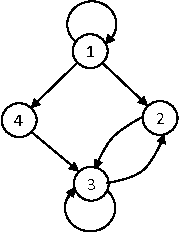
\includegraphics[scale=0.9]{Graficos/fig1_RB}		}{  \caption*{Grafo \(R\)}	}
	%
\end{floatrow}
\end{figure}
%
\end{ejem}

\paragraph{Relaciones derivadas.}

Sea \(R\) una relación sobre el conjunto \(X\), la relación inversa \(R^{-1}\), el complemento \(R^{c}\) de la relación \(R\) se definen por:
\begin{align*}
    R^{-1} &= \big\{(x,y) \in X : \,(y,x) \in R \big\} \\
    R^{c} &= \big\{(x,y) \in X : \, (y,x) \not \in R\big\} 
\end{align*}

\paragraph{Relación identidad.}

Relaciones identidad es:
\[
	I_d = \big\{ (x,x) : \, x \in X \big\}
\]

\vspace{-1\baselineskip}
\paragraph{Composición de relaciones.}

Si \(R\) y \(T\) son dos relaciones sobre \(X\), la relación compuesta \(RT\) se define por: \(x \, RT \, y\) ssi para algún \(z \in X, \; x \, R\, z \wedge z \, T\, y\).

%
\begin{ejem}

Sean \(R\) y \(T\) las relaciones definidas por las siguientes matrices:

%
\begin{table}[H]
	\fontsize{7}{11}\selectfont
    %\caption{Global caption}
    \begin{minipage}{.5\linewidth}
      %\caption{}
      \centering
	\begin{tabular}{c|ccccc} \thickline
	\(R\) & \(A_1\) & \(A_2\) & \(A_3\) & \(A_4\) & \(A_5\)  \\	\hline
    \(A_1\) & 1 & 1 & 0 & 1 & 1  \\
    \(A_2\) & 0 & 1 & 1 & 0 & 1  \\
	\(A_3\) & 0 & 1 & 0 & 1 & 0   \\
	\(A_4\) & 1 & 0 & 1 & 0 & 1   \\
	\(A_5\) & 0 & 0 & 1 & 0 & 1   \\
\end{tabular}
\label{tab:B2} 
    \end{minipage}%
    \begin{minipage}{.5\linewidth}
      \centering
        %\caption{}
	\begin{tabular}{c|ccccc} \thickline
	\(T\) & \(A_1\) & \(A_2\) & \(A_3\) & \(A_4\) & \(A_5\)  \\	\hline
    \(A_1\) & 0 & 1 & 0 & 1 & 0  \\
    \(A_2\) & 0 & 0 & 1 & 0 & 0  \\
	\(A_3\) & 1 & 0 & 0 & 1 & 0   \\
	\(A_4\) & 0 & 0 & 0 & 1 & 1   \\
	\(A_5\) & 1 & 1 & 0 & 0 & 1   \\
\end{tabular}
\label{tab:B3}
    \end{minipage} 
\end{table}
%

%\vfill
%\newpage

Entonces

\begin{table}[H]
   \fontsize{7}{11}\selectfont
    \begin{minipage}{.5\linewidth}
      \centering
	\begin{tabular}{c|ccccc} \thickline
	\(R^{-1}\) & \(A_1\) & \(A_2\) & \(A_3\) & \(A_4\) & \(A_5\)  \\
	\hline
    \(A_1\) & 1 & 0 & 0 & 1 & 0  \\
    \(A_2\) & 1 & 1 & 1 & 0 & 0  \\
	\(A_3\) & 0 & 1 & 0 & 1 & 1   \\
	\(A_4\) & 1 & 0 & 1 & 0 & 0   \\
	\(A_5\) & 1 & 1 & 0 & 1 & 1   \\
\end{tabular}
\label{tab:B4} 
    \end{minipage}%
    \begin{minipage}{.5\linewidth}
      \centering
        %\caption{}
	\begin{tabular}{c|ccccc} \thickline
	\(R^{c}\) & \(A_1\) & \(A_2\) & \(A_3\) & \(A_4\) & \(A_5\)  \\
	\hline
    \(A_1\) & 0 & 0 & 1 & 0 & 0  \\
    \(A_2\) & 1 & 0 & 0 & 1 & 0  \\
	\(A_3\) & 1 & 0 & 1 & 0 & 1   \\
	\(A_4\) & 0 & 1 & 0 & 1 & 0   \\
	\(A_5\) & 1 & 1 & 0 & 1 & 0   \\
\end{tabular}
\label{tab:B5} 
    \end{minipage} 
\end{table}


\begin{table}[H]
\fontsize{7}{11}\selectfont
\begin{center}
	\begin{tabular}{c|ccccc} \thickline
	\(RT\) & \(A_1\) & \(A_2\) & \(A_3\) & \(A_4\) & \(A_5\)  \\
	\hline
    \(A_1\) & 1 & 1 & 1 & 1 & 1  \\
    \(A_2\) & 1 & 0 & 0 & 1 & 0  \\
	\(A_3\) & 0 & 0 & 1 & 1 & 1   \\
	\(A_4\) & 1 & 1 & 0 & 1 & 0   \\
	\(A_5\) & 1 & 1 & 0 & 1 & 1   \\
\end{tabular}
\label{tab:B6} 
\end{center}
\end{table}
\end{ejem}

\textbf{Observación:} La matriz asociada a \(RT\) es el producto booleano \footnote{La suma y el producto booleano se definen por: \(0+0 = 0\), \( 0+1 = 1+0 = 1\), \(1+1 = 1\); \( 0\times0 = 0\), \( 0\times1 = 1\times0 = 0\), \( 1\times 1 = 1\).} de las matrices \(R\) y \(T\).\\

Para simplificar la escritura escribimos <<ssi>> en lugar de <<si y solo si>>.

\paragraph{Propiedades de las relaciones.}

Se dice que la relación \(R\) satisface la propiedad:

\begin{table}[H]
\fontsize{7.5}{11}\selectfont
\begin{center}
\begin{tabular}{l l l l l}
	Reflexiva & ssi & \(x \, R \, x\) & ssi & \(I_d \subset R\)  \\
    Irreflexiva & ssi & \( \neg(x \, R \, x)\) & ssi & \(R \subset I_d^{c}\)  \\
    Simétrica & ssi & \( (x \, R \, y) \Longrightarrow (y \, R \, x)\) & ssi & \(R = R^{-1}\)  \\
    Asimétrica & ssi & \( (x \, R \, y) \Longrightarrow \neg (y \, R \, x)\) & ssi & \(R \cap R^{-1} = \varnothing \)  \\
    Antisimétrica & ssi & \( (x \, R \, y) \wedge (y \, R \, x) \Longrightarrow (x = y)\) & ssi & \(R \cap R^{-1} = I_d\)  \\
    Transitiva & ssi & \( (x \, R \, y) \wedge (y \, R \, z) \Longrightarrow (x \, R \, z)\) & ssi & \(RR \subset R\)  \\
    Semitransitiva & ssi & \( (x \, R \, y) \wedge (y \, R \, z) \Longrightarrow (x \, R \, u) \vee (u \, R \, z) \) & ssi & \(PPI \subset P\) \; \text{ssi} \; \(IPP \subset P\) \\
    Ferrers & ssi & \( (x \, R \, y) \wedge (z \, R \, u) \Longrightarrow (x \, R \, u) \vee (z \, R \, y) \) & ssi & \(PIP \subset P\)\\
    Completa & ssi & \( (x \, R \, y) \vee (y \, R \, x) \) & ssi & \(X^2 = R \cup R^{-1}\)  \\
    Cuasi completa & ssi & \( x \neq y \Longrightarrow (x \, R \, y) \vee (y \, R \, x) \) & ssi & \(X^2 \backslash I_d = R \cup R^{-1}\)  \\[-2\baselineskip]
\end{tabular}
\label{tab:B7} 
\end{center}
\end{table}



Para todo \(x,y,z,u \in X\), según corresponda.

La completitud y cuasi completitud se denominan también completitud fuerte y completitud
respectivamente \citeA{Ozturke-2003}.

%\newpage

\paragraph{Relaciones de orden.}

Sean \(I\), \(P\) y \(R\) relaciones definidas sobre el conjunto \(X\). Se dice que \(R\) es una relación de:

\begin{table}[H]
\fontsize{8}{11}\selectfont
\begin{center}
\begin{tabular}{l l l }
	Orden parcial      & ssi & \(R\) es reflexiva, antisimétrica y transitiva  \\
	                   & ssi & \(I_d \subset R\), \( R \cap R^{-1} \subset I_d \) y \(RR \subset R \)\\
    Pre-orden parcial  & ssi & \(R\) es reflexiva y transitiva \\
                       & ssi & \(I_d \subset R\) y \(RR \subset R \)\\
    Semi-orden parcial & ssi & \(R\) es reflexiva, Ferrers y semitransitiva \\
                       & ssi & \(I_d \subset R\), \(PIP \subset P\) y \(PPI \subset P \)\\[-1\baselineskip]
\end{tabular}
\label{tab:B8} 
\end{center}
\end{table}

\vspace{-1\baselineskip}

Una relación de orden, preorden o semiorden parcial es una relación de orden, preorden o semiorden total ssi la relación es completa ssi \(X^2 = R \cup R^{-1}\).

La relación \(P\) se denomina:

\begin{table}[H]
\fontsize{7.5}{11}\selectfont
\begin{center}
	\begin{tabular}{l l l }
		Orden estricto parcial & si & \(P\) es asimétrica y transitiva \\
	    	                   & ssi & \(P \cap P^{-1} = \varnothing \) y \(PP \subset P \)\\[-1\baselineskip]
	\end{tabular}
	\label{tab:B9} 
\end{center}
\end{table}

\vspace{-1\baselineskip}

Una relación de orden estricta parcial es una relación de orden estricta total ssi la relación es cuasi-completa ssi \(X^2  \backslash  I_d = R \cup R^{-1}\).

El par \((X,R)\) o \((X,P)\) se denomina estructura de orden.

La relación \(I\) se denomina de:

\begin{table}[H]
\fontsize{7.5}{11}\selectfont
\begin{center}
	\begin{tabular}{l l l }
		Semejanza & si & \(I\) es reflexiva y simétrica \\
	    	      & ssi & \(I_d \subset I \), \(I = I^{-1} \)\\
		Equivalencia & si & \(I\) es reflexiva, simétrica y transitiva \\
	          	     & ssi & \(I_d \subset I \), \(I = I^{-1} \) y \(II \subset I\)\\[-1\baselineskip]
	\end{tabular}
\label{tab:B10} 
\end{center}
\end{table}

\vspace{-1\baselineskip}

La clase de equivalencia de \(x \in X\) para la relación de equivalencia \(I\), se define por:
\[
	[x] = \big\{y \in X : x \, I \, y \big\}
\]

\textbf{Observación:}

\begin{APAenumerate}
    \item La completitud implica la reflexividad; la asimetría la irreflexividad; y, la completitud implica la cuasi-completitud.
    \item La completitud es un supuesto de partida en la economía convencional (mainstream). La economía ecológica por el contrario considera la comparabilidad débil de valores como uno de sus fundamentos (Alier et al 1998). Siendo este el caso, queda abierta completamente la posibilidad de no comparabilidad entre alternativas, lo que lleva a estructuras de orden parcial.
\end{APAenumerate}


%\vfill
%\newpage

Ejemplos de las distintas estructuras de orden.


%\vspace{1\baselineskip}
\begin{ejem} Orden total

\begin{table}[H]
\begin{floatrow}
	\fontsize{7}{11}\selectfont
	\captionsetup{justification=centering, labelfont=footnotesize, font=footnotesize}
	%	Tabla
	\capbtabbox{%
	 \begin{tabular}{c|cccc} \thickline
	\(R\) & \(A_1\) & \(A_2\) & \(A_3\) & \(A_4\)   \\ \hline
    \(A_1\) & 1 & 0 & 0 & 1  \\
    \(A_2\) & 1 & 1 & 1 & 1  \\
	\(A_3\) & 1 & 0 & 1 & 1  \\
	\(A_4\) & 0 & 0 & 0 & 1  \\
	\end{tabular}
	\vspace{0.35cm}
	}{	  %\caption*{Matriz \(R\) \\ El nodo \(A_i\) se etiqueta únicamente \(i\).}%
	}
	\capbtabbox{%
	 \begin{tabular}{c|cccc} \thickline
	\(R\) & \(A_2\) & \(A_3\) & \(A_1\) & \(A_4\)   \\ \hline
    \(A_2\) & 1 & 1 & 1 & 1  \\
    \(A_3\) & 0 & 1 & 1 & 1  \\
	\(A_1\) & 0 & 0 & 1 & 1  \\
	\(A_4\) & 0 & 0 & 0 & 1  \\
	\end{tabular}
	}{	  \caption*{(reordenando \(X\))}%
	}
\end{floatrow}
\end{table}

\[
	R: A_2 > A_3 > A_1 > A_4
\]

\begin{figure}[H]
    \centering
    
\includegraphics[scale=0.9]{Graficos/fig2_RB}
    \label{fig:RB_grafo2}
\end{figure}

\end{ejem}

En un orden total finito los elementos pueden ordenarse uno detrás de otro, por ello se lo denomina también orden lineal. La relación \(P = R \backslash I\) es un orden estricto.

Para visibilizar de mejor manera, en un grafo no se grafican los arcos que se pueden obtenerse por la aplicación de la transitividad. Así en un orden lineal se suele graficar únicamente los arcos que enlazan un nodo al siguiente.

El ejemplo paradigmático de orden total es el orden usual <<mayor o igual>> (\(\geq\)) en los números naturales o en los números reales.

\newpage

\vspace{1\baselineskip}
\begin{ejem} Preorden 

\begin{table}[H]
\begin{floatrow}
	\fontsize{7}{11}\selectfont
	\captionsetup{justification=centering, labelfont=footnotesize, font=footnotesize}
	%	Tabla
	\capbtabbox{%
	 \begin{tabular}{c|ccccc} \thickline
	\(R\) & \(A_1\) & \(A_2\) & \(A_3\) & \(A_4\) & \(A_5\)    \\ \hline
    \(A_1\) & 1 & 0 & 0 & 1 & 0  \\
    \(A_2\) & 1 & 1 & 0 & 1 & 0  \\
	\(A_3\) & 1 & 1 & 1 & 1 & 1  \\
	\(A_4\) & 1 & 0 & 0 & 1 & 0  \\
	\(A_5\) & 1 & 1 & 1 & 1 & 1  \\
	\end{tabular}
	\vspace{0.35cm}
	}{	  %\caption*{Matriz \(R\) \\ El nodo \(A_i\) se etiqueta únicamente \(i\).}%
	}
	\capbtabbox{%
	 \begin{tabular}{c|ccccc} \thickline
	\(R\) & \(A_3\) & \(A_5\) & \(A_2\) & \(A_1\) & \(A_4\)    \\ 	\hline
    \(A_3\) & 1 & 1 & 1 & 1 & 1  \\
    \(A_5\) & 1 & 1 & 1 & 1 & 1  \\
	\(A_2\) & 0 & 0 & 1 & 1 & 1   \\
	\(A_1\) & 0 & 0 & 0 & 1 & 1  \\
	\(A_4\) & 0 & 0 & 0 & 1 & 1  \\
	\end{tabular}
	}{	  \caption*{(reordenando \(X\))}%
	}
\end{floatrow}
\end{table}

\[
	R: A_3 = A_5 > A_2 > A_1 = A_4
\]

\begin{figure}[H]
    \centering
    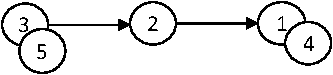
\includegraphics[scale=0.9]{Graficos/fig3_RB}
    \label{fig:RB_grafo2}
\end{figure}

Reordenando los elementos de \(X\) de ser necesario, la matriz de una relación de preorden es una matriz con 1’s en la triangular superior y una estructura de bloques cuadrados de 1’s disjuntos sobre la diagonal principal. Los bloques cuadrados determinan a las clases de equivalencia, pues \(I\) es una relación de equivalencia. En el ejemplo: \([A_3] = \{A_3, A_5\}\), \([A_2] = \{A_2\}\), \([A_1] = \{A_1, A_4\}\) y están totalmente ordenadas por la relación inducida \([x] \, R \, [y]\) si \( x \, R \, y\). En el ejemplo, \([A_3] \, R \, [A_2] \,  R \, [A_1]\). Las clases de equivalencia forman una partición de \(X\) (las clases de equivalencia son disjuntas y su unión es igual a \(X\)).

\end{ejem}

%\vspace{1\baselineskip}
En la microeconomía se asume que las preferencias de los consumidores son un preorden sobre el conjunto de canastas de consumo; las <<curvas de indiferencia>> son las clases de equivalencia.

\begin{ejem} Semiorden 

\begin{table}[H]
\begin{floatrow}
	\fontsize{7}{11}\selectfont
	\captionsetup{justification=centering, labelfont=footnotesize, font=footnotesize}
	%	Tabla
	\capbtabbox{%
	 \begin{tabular}{c|ccccc} \thickline
	\(R\) & \(A_1\) & \(A_2\) & \(A_3\) & \(A_4\) & \(A_5\)    \\ \hline
    \(A_1\) & 1 & 0 & 1 & 1 & 1  \\
    \(A_2\) & 1 & 1 & 1 & 1 & 1  \\
	\(A_3\) & 1 & 0 & 1 & 0 & 0  \\
	\(A_4\) & 1 & 1 & 1 & 1 & 1  \\
	\(A_5\) & 1 & 1 & 1 & 1 & 1  \\
	\end{tabular}
	\vspace{0.9\baselineskip}
	}{	  %\caption*{Matriz \(R\) \\ El nodo \(A_i\) se etiqueta únicamente \(i\).}%
	}
	\capbtabbox{%
	 \begin{tabular}{c|ccccc} \thickline
	\(R\) & \(A_2\) & \(A_4\) & \(A_5\) & \(A_1\) & \(A_3\)    \\ 	\hline
    \(A_2\) & 1 & 1 & 1 & 1 & 1  \\
    \(A_4\) & 1 & 1 & 1 & 1 & 1  \\
	\(A_5\) & 1 & 1 & 1 & 1 & 1  \\
	\(A_1\) & 0 & 1 & 1 & 1 & 1  \\
	\(A_3\) & 0 & 0 & 0 & 1 & 1  \\
	\end{tabular}
	}{	  \caption*{(reordenando \(X\))}%
	}
\end{floatrow}
\end{table}

\vspace{-1\baselineskip}
\begin{figure}[H]
    \centering
    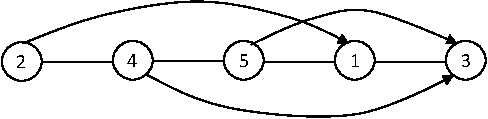
\includegraphics[scale=0.9]{Graficos/fig4_RB}
    \label{fig:RB_grafo4}
\end{figure}

En un semiorden, al reordenar los elementos de \(X\) de ser necesario, la matriz asociada tiene 1’s en la triangular superior y una estructura de bloques cuadrados de 1’s no necesariamente disjuntos sobre la diagonal principal. La matriz asociada es en <<escalera>>: la frontera entre los 0’s y 1’s tiene la forma de una escalera con los 0’s en la triangular inferior de la matriz \cite{Monjardet-1978}.

La relación \(I\) es una relación de semejanza. No es una relación transitiva.

\end{ejem}

En el grafo de un semiorden, los nodos se pueden graficar en secuencia, uno a continuación de otro (o uno debajo de otro), siguiendo el orden de los elementos en la matriz en escalera. Cada nodo se enlaza con el primer nodo estrictamente menor mediante un arco dirigido (flecha). El nodo <<padre>> será mayor al nodo hijo y a todos los nodos a la derecha (o inferiores). Esto permite graficar un conjunto limitado de arcos y visibilizar de mejor manera el grafo.

En el ejemplo, los bloques son: \(B_1 = \{A_2, A_4, A_5\}\), \(B_2 = \{A_4, A_5, A_1\}\), \(B_3 = \{A_1, A_3\}\). No son clases de equivalencia pues no son bloques disjuntos, pero son bloques consecutivos.

Nótese que en un semiorden los mejores elementos de \(X\) son los elementos de \(B_1 \backslash \cup _{i \geq 2} B_i\). Los elementos de este conjunto son máximos, satisfacen que para todo \(y \in X\), \(x \, R \, y\).

\vspace{1\baselineskip}
Un semiorden es una estructura adecuada para modelar y evitar la <<paradoja de Luce>> en la microeconomía tradicional: Un consumidor prefiere estrictamente una taza de café con dos cucharadas de azúcar (\(10 [gr]\)) a una taza de café sin azúcar. Por otra parte, el consumidor es indiferente entre dos tazas de café con \(z\) y \(z + \epsilon\) gramos de azúcar (\(0 \geq z \geq 10\); \(\epsilon = 0.01\)). Si se forma la cadena indiferencia de tazas de café con: \(0\); \(0,01\); \(0,02\); \(\dots\); \(9,98\); \(9,99\); \(10\) gramos de azúcar; al final se concluirá que el consumidor es indiferente entre la taza de café con \(10 [gr]\) de azúcar y la taza de café sin azúcar.

\begin{ejem} Orden parcial

\begin{figure}[H]
\begin{floatrow}
	\fontsize{7}{11}\selectfont
	\captionsetup{justification=centering, labelfont=footnotesize, font=footnotesize}
	%	Tabla
	\capbtabbox{%
	 \begin{tabular}{c|cccc} \thickline
	\(R\) & \(A_2\) & \(A_3\) & \(A_1\) & \(A_4\) \\ \hline
    \(A_2\) & 1 & 1 & 1 & 0   \\
    \(A_3\) & 0 & 1 & 0 & 1   \\
	\(A_1\) & 0 & 0 & 1 & 1   \\
	\(A_4\) & 0 & 0 & 0 & 1   \\
	\end{tabular}
	\vspace{2em}
	}{	  \caption*{}%
	}
	%	Figura
	\ffigbox{	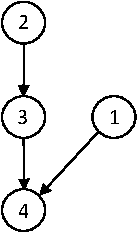
\includegraphics[scale=0.75]{Graficos/fig5_RB}		}{  \caption*{}	}
	%
\end{floatrow}
\end{figure}

\vspace{-2\baselineskip}
La estructura de orden parcial es bastante común. Por ejemplo, los elementos de una familia de subconjuntos de un conjunto están relacionados por un orden parcial

\end{ejem}

\newpage

\begin{ejem} Preorden parcial

\vspace{1\baselineskip}
\begin{figure}[H]
\begin{floatrow}
	\fontsize{7}{11}\selectfont
	\captionsetup{justification=centering, labelfont=footnotesize, font=footnotesize}
	%	Tabla
	\capbtabbox{%
	 \begin{tabular}{c|ccccc} \thickline
	\(R\) & \(A_3\) & \(A_5\) & \(A_2\) & \(A_1\) & \(A_4\)     \\ \hline
    \(A_3\) & 1 & 1 & 1 & 1 & 1  \\
    \(A_5\) & 1 & 1 & 1 & 1 & 1  \\
	\(A_2\) & 0 & 0 & 1 & 0 & 0  \\
	\(A_1\) & 0 & 0 & 0 & 1 & 1  \\
	\(A_4\) & 0 & 0 & 0 & 1 & 1  \\
	\end{tabular}
	}{	  \caption*{}%
	}
	%	Figura
	%\vspace{-1\baselineskip}
	\ffigbox{	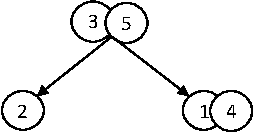
\includegraphics[scale=0.75]{Graficos/fig6_RB}		}{  \caption*{}	}
	%
\end{floatrow}
\end{figure}

\end{ejem}

\begin{ejem} Semiorden parcial

\vspace{-2.3\baselineskip}
\begin{figure}[H]
\begin{floatrow}
	\fontsize{7}{11}\selectfont
	\captionsetup{justification=centering, labelfont=footnotesize, font=footnotesize}
	%	Tabla
	\capbtabbox{%
	 \begin{tabular}{c|ccccc} \thickline
	\(R\) & \(A_2\) & \(A_4\) & \(A_5\) & \(A_1\) & \(A_3\)    \\ 	\hline
    \(A_2\) & 1 & 0 & 1 & 1 & 1  \\
    \(A_4\) & 0 & 1 & 1 & 1 & 1  \\
	\(A_5\) & 0 & 1 & 1 & 1 & 1  \\
	\(A_1\) & 0 & 0 & 1 & 1 & 1  \\
	\(A_3\) & 0 & 0 & 0 & 1 & 1  \\
	\end{tabular}
	\vspace{2em}
	}{	  \caption*{}%
	}
	%	Figura
	\ffigbox{	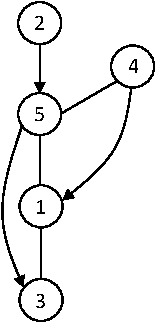
\includegraphics[scale=0.75]{Graficos/fig7_RB}		}{  \caption*{}	}
	%
\end{floatrow}
\end{figure}

\end{ejem}

%\vfill
%\newpage

\vspace{-2\baselineskip}

\subsubsection{Estructura \(I-P-J\).}

La tripleta \(I\), \(P\), \(J\) de relaciones sobre \(X\) se denomina una estructura de preferencia \(I-P-J\) ssi satisface las condiciones:

\vspace{1\baselineskip}
\begin{APAenumerate}
    \item \(I\) es reflexiva y simétrica.
    \item \(P\) es asimétrica.
    \item \(J\) es irreflexiva y simétrica.
    \item \(P \cap I = P \cap J = I \cap J = \varnothing\).
    \item \(X^2 = I \cup P \cup P^{-1} \cup J\). 
    \item La relación característica o relación grande \(R\) se define por \(R = I \cup P\)
\end{APAenumerate}

\vspace{1\baselineskip}
Si \(J = \varnothing\), la estructura de preferencia se denomina estructura \(I-P\).

\newpage

\begin{ejem}
Para la relación \(R\) del ejemplo 2. Se tiene que:

\begin{table}[H]
	\fontsize{7}{11}\selectfont
    %\caption{Global caption}
    \begin{minipage}{.5\linewidth}
      %\caption{}
      \centering
	\begin{tabular}{c|ccccc} \thickline
	\(R\) & \(A_1\) & \(A_2\) & \(A_3\) & \(A_4\) & \(A_5\)  \\ \hline
    \(A_1\) & 1 & 1 & 0 & 1 & 1  \\
    \(A_2\) & 0 & 1 & 0 & 0 & 1  \\
	\(A_3\) & 0 & 1 & 1 & 1 & 0   \\
	\(A_4\) & 1 & 0 & 1 & 1 & 1   \\
	\(A_5\) & 0 & 0 & 1 & 0 & 1   \\
\end{tabular}
\label{tab:B2} 
    \end{minipage}%
    \begin{minipage}{.5\linewidth}
      \centering
        %\caption{}
	\begin{tabular}{c|ccccc} \thickline
	\(R^{-1}\) & \(A_1\) & \(A_2\) & \(A_3\) & \(A_4\) & \(A_5\)  \\ \hline
    \(A_1\) & 1 & 1 & 0 & 1 & 1  \\
    \(A_2\) & 0 & 1 & 1 & 0 & 1  \\
	\(A_3\) & 0 & 0 & 1 & 1 & 0   \\
	\(A_4\) & 1 & 0 & 1 & 1 & 1   \\
	\(A_5\) & 0 & 0 & 1 & 0 & 1   \\
\end{tabular}
\label{tab:B3}
    \end{minipage} 
\end{table}
%

\begin{table}[H]
   \fontsize{7}{11}\selectfont
    \begin{minipage}{.5\linewidth}
      \centering
	\begin{tabular}{c|ccccc} \thickline
	\(I\) & \(A_1\) & \(A_2\) & \(A_3\) & \(A_4\) & \(A_5\)  \\ \hline
    \(A_1\) & 1 & 0 & 0 & 1 & 0  \\
    \(A_2\) & 0 & 1 & 0 & 0 & 0  \\
	\(A_3\) & 0 & 1 & 1 & 1 & 0   \\
	\(A_4\) & 1 & 0 & 1 & 1 & 0   \\
	\(A_5\) & 0 & 0 & 0 & 0 & 1   \\
\end{tabular}
\label{tab:B4} 
    \end{minipage}%
    \begin{minipage}{.5\linewidth}
      \centering
        %\caption{}
	\begin{tabular}{c|ccccc} \thickline
	\(P\) & \(A_1\) & \(A_2\) & \(A_3\) & \(A_4\) & \(A_5\)  \\ \hline
    \(A_1\) & 0 & 1 & 0 & 0 & 1  \\
    \(A_2\) & 0 & 0 & 0 & 0 & 1  \\
	\(A_3\) & 0 & 1 & 0 & 0 & 0   \\
	\(A_4\) & 0 & 0 & 0 & 0 & 1   \\
	\(A_5\) & 0 & 0 & 1 & 0 & 0   \\
\end{tabular}
\label{tab:B5} 
    \end{minipage} 
\end{table}

%

\begin{table}[H]
   \fontsize{7}{11}\selectfont
    \begin{minipage}{.5\linewidth}
      \centering
	\begin{tabular}{c|ccccc} \thickline
	\(P^{-1}\) & \(A_1\) & \(A_2\) & \(A_3\) & \(A_4\) & \(A_5\)  \\ \hline
    \(A_1\) & 0 & 0 & 0 & 0 & 0  \\
    \(A_2\) & 1 & 0 & 1 & 0 & 0  \\
	\(A_3\) & 0 & 0 & 0 & 0 & 1   \\
	\(A_4\) & 0 & 0 & 0 & 0 & 0   \\
	\(A_5\) & 1 & 1 & 0 & 1 & 0   \\
\end{tabular}
\label{tab:B4} 
    \end{minipage}%
    \begin{minipage}{.5\linewidth}
      \centering
        %\caption{}
	\begin{tabular}{c|ccccc} \thickline
	\(J\) & \(A_1\) & \(A_2\) & \(A_3\) & \(A_4\) & \(A_5\)  \\ \hline
    \(A_1\) & 0 & 0 & 1 & 0 & 0  \\
    \(A_2\) & 0 & 0 & 0 & 1 & 0  \\
	\(A_3\) & 1 & 0 & 0 & 0 & 0   \\
	\(A_4\) & 0 & 1 & 0 & 0 & 0   \\
	\(A_5\) & 0 & 0 & 0 & 0 & 0   \\
\end{tabular}
\label{tab:B5} 
    \end{minipage} 
\end{table}

\end{ejem}

\subsubsection{Matriz de relaciones o matriz coloreada.}

La información anterior puede resumirse en la matriz de relaciones definida por:
\begin{align*}
    R_0 : X \times X & \longrightarrow \big\{I, P , P^{-1}, J \big\} \\
    (x,y) & \mapsto R_0(x,y) = \text{argmax} \big\{R_k(x,y)\big\}
\end{align*}

Es decir, a cada par \((x,y)\) se le asocia el símbolo de la relación que se satisface en el par. Para destacar las relaciones se pinta o colorea el fondo de la celda con: amarillo para la indiferencia, celeste para la preferencia estricta, verde para la preferencia estricta inversa, y gris para la indiferencia.

\newpage

\begin{ejem} Continuando con el ejemplo 9.

\begin{table}[H]
   \fontsize{7}{11}\selectfont
   	\captionsetup{justification=centering, labelfont=footnotesize, font=footnotesize}
    \centering
	\begin{tabular}{c|ccccc} \thickline
	\(R_0\) & \(A_1\) & \(A_2\) & \(A_3\) & \(A_4\) & \(A_5\)  \\ \hline
    \(A_1\) & \cellcolor{pastelyellow} I & \cellcolor{paleblue} P & \cellcolor{pastelgray}J & \cellcolor{pastelyellow} I & \cellcolor{paleblue} P  \\
    \(A_2\) &  & \cellcolor{pastelyellow} I & \cellcolor{palegreen} \(P^{-1}\) & \cellcolor{pastelgray}J & \cellcolor{paleblue} P  \\
	\(A_3\) &  &  & \cellcolor{pastelyellow} I & \cellcolor{pastelyellow} I & \cellcolor{palegreen} \(P^{-1} \)  \\
	\(A_4\) &  &  &  & \cellcolor{pastelyellow} I & \cellcolor{paleblue} P   \\
	\(A_5\) &  &  &  &  & \cellcolor{pastelyellow}I   \\
    \end{tabular}
    \caption*{Matriz coloreada}
\label{tab:B4} 
\end{table}
\end{ejem}

	\subsection{Conjuntos difusos.}

En un conjunto <<clásico>>, no difuso, dado un conjunto \(A\) y un elemento \(x\), se tiene que: \(x\) pertenece a \(A\) o, \(x\) no pertenece a \(A\). Por ejemplo si \(A = \{x : x \, \text{es alto}\}\) y \(x = \text{Jorge}\), se tiene que Jorge es alto o Jorge no es alto. Si, digamos, Jorge mide \(1.90 [m]\) (y lo consideramos alto), ¿qué se puede decir de Santiago que mide \(1.85 [m]\) y de María que mide \(1.60[m]\)?

Posiblemente la respuesta sea: Santiago es medianamente alto, María es muy poco alta. Los conjuntos difusos permiten expresar estas ideas. En los conjuntos clásicos se puede definir una función de pertenencia al conjunto \(A\) que toma el valor 1 si \(x \in A\) y vale 0 si \(x \not \in A\) (y solo toma estos valores). En los conjuntos difusos, la función grado de pertenencia al conjunto difuso \(A\) puede ser cualquier valor entre 0 y 1. El grado de pertenencia igual a 0 significará que es absoluta y totalmente certero que \(x \not \in A\). El grado de pertenencia igual a 1 significará que es absoluta y totalmente certero que \(x \in A\). Así, para el conjunto difuso \(A\) (el conjunto de los altos), se tendrá que \(\text{gr}(\text{Jorge} \in A) = 1\); \(\text{gr}(\text{Santiago} \in A) = 0.90\); \(\text{gr}(\text{María} \in A) = 0.30\). Veamos ahora la definición formal de conjunto difuso. 

\subsubsection{Conjuntos difusos.}

Sea \(X\) un conjunto cualesquiera que lo denominaremos universo del discurso.

\begin{APAitemize}
    \item Un conjunto difuso \(A\) es una función \(\mu _A: X \rightarrow [0,1]\) que para cada elemento de \(x \in X\) asocia el grado de pertenencia, o la credibilidad de la pertenencia, de \(x\) al conjunto \(A\). Se nota \(\mu _A(x) = \text{gr}(x \in A)\).
    
    \item Una relación difusa \(R\) sobre \(X\) es un subconjunto difuso en \(X \times X\). El grado de pertenencia del par \((x,y) \in X \times X\) al conjunto \(R\) se nota \(R(x,y)\). Se dice también que \(R(x,y)\) el grado de credibilidad, o simplemente credibilidad, de la relación \(R(x,y)\).
\end{APAitemize}

\subsubsection{Operaciones entre conjuntos difusos.}

Las operaciones clásicas entre conjuntos: unión, intersección y complemento se extienden a los conjuntos difusos de la siguiente manera:

\paragraph{Complemento.}

Un complemento difuso de un conjunto difuso \(A\) es una función \(N\) que al grado de pertenencia al conjunto difuso \(A\) le asocia el grado de pertenencia al conjunto difuso complemento \(A^{c}\).
    \begin{align*}
    N: [0,1] & \longrightarrow [0,1]\\
    \mu _A(x) & \longrightarrow N(\mu _A(x)) = \mu _{A^{c}}(x)
    \end{align*}

Cumple las condiciones siguientes:
\begin{align*}
	\text{condiciones de borde:	}&	& N(0) &= 1,\qquad  N(1) = 0,
	\\
	\text{monotonía creciente:		}&	& a&<b	\Rightarrow N(a) \geq N(b).
\end{align*}

Adicionalmente se puede exigir el cumplimiento de las condiciones siguientes:
\begin{APAitemize}
    \item \(N\) es una función continua.
    \item \(N\) es estrictamente decreciente, en tal caso se denomina negación estricta.
    \item \(N\big(N(a)\big) = a\), involución. De ser este el caso se denomina negación fuerte.
\end{APAitemize}

\paragraph{Intersección.}
La intersección difusa de dos conjuntos difusos \(A\) y \(B\) es una función \(T\), denominada norma triangular o t-norma, que al par de grados de pertenencia de un elemento a los conjuntos \(A\) y \(B\) le asocia el grado de pertenencia al conjunto difuso intersección \(A \cap _T B\).
    \begin{align*}
    T: [0,1] \times [0,1] & \longrightarrow [0,1]\\
    (\mu _A(x), \mu _B(x)) & \longrightarrow T(\mu _A(x), \mu _B(x)) = \mu_{A\cap B} (x)
    \end{align*}

Cumple las condiciones:
\begin{align*}
	T(1,a) &= a 		&	\text{condiciones de borde}	\\
	T(a,b) &= T(b,a) 	&	\text{conmutatividad}			\\
	a \leq a' \wedge b \leq b' &\Rightarrow T(a,b) \leq T(a',b')	&	\text{monotonía no decreciente}			\\
	T\big(T(a,b),c\big) &= T\big(a, T(b,c)\big)	&		\text{asociatividad}			\\
\end{align*}

    
Adicionalmente se puede exigir el cumplimiento de la condición:

\begin{center}
	\(T\) es una función continua.
\end{center}

\paragraph{Unión.}

La unión difusa de dos conjuntos difusos \(A\) y \(B\) es una función \(S\), denomina co-norma triangular o t-conorma o s-norma, que al par de grados de pertenencia a \(A\) y \(B\) le asocia el grado de pertenencia al conjunto difuso unión  \(A \cup _S B\).
    \begin{align*}
    S: [0,1] \times [0,1] & \longrightarrow [0,1]\\
    (\mu _A(x), \mu _B(x)) & \longrightarrow S(\mu _A(x), \mu _B(x)) = \mu_{A\cup B} (x)
    \end{align*}

Cumple las condiciones:
\begin{align*}
	S(0,a) &= a 		&	\text{condiciones de borde}	\\
	S(a,b) &= S(b,a) 	&	\text{conmutatividad}			\\
	a \leq a' \wedge b \leq b' &\Rightarrow S(a,b) \leq S(a',b')	&	\text{monotonía no decreciente}			\\
	S\big(S(a,b),c\big) &= S\big(a, S(b,c)\big)	&		\text{asociatividad}			\\
\end{align*}
 
Adicionalmente se puede exigir el cumplimiento de la condición:

\begin{center}
	\(S\) es una función continua.
\end{center}

\newpage
\begin{ejem}

\begin{APAenumerate}
    \item La negación usual es la función \(N(a)=1-a\).
    \item La t-norma y la t-conorma de Frank de parámetro \(s\), son:
    \begin{align*}
    	T^s(a,b) & = \log _s \left(1+\dfrac{(s^a -1)(s^b-1)}{s-1}\right),			\\	
    	S^s(a,b) & = 1- \log _s \left(1+\dfrac{(s^{1-a} -1)(s^{1-b}-1)}{s-1}\right), 	\qquad s \in (0,\infty).
    \end{align*}

    \item La t-norma y la t-conorma de Lukasiewics son:
    \begin{align*}
    	T(a,b) & = \max (a+b-1,0),		\\
    	S(a,b) & = \min (a+b,1).
    \end{align*}    
    
\end{APAenumerate}
\end{ejem}

\textbf{Observación:} La negación usual, la t-norma y la t-conorma de Frank de parámetro \(s\); la negación usual, la t-norma y la t-conorma de Lukasiewics son tripletas de De Morgan; es decir, satisfacen las leyes de De Morgan:
\begin{align*}
	(A \cup_S B)^c &= A^c \cap_T B^c	,
	\\
	(A \cap_T B)^c &= A^c \cup_S B^c	.
\end{align*}

La t-norma y la t-conorma de Frank de parámetro \(s\), satisface que:
    \begin{align*}
    	\lim _{s \rightarrow 1} T^s(a,b) & = T^1(a,b)  = ab,	\\
    	\lim _{s \rightarrow \infty} S^s(a,b) & = S^{\infty} (a,b)  = \min (a+b,1).
    \end{align*}  

\subsubsection{Estructura \(I-P-J\) difusa.}

En el modelo no difuso, a partir de la preferencia débil \(R\) las relaciones \(I\), \(P\), \(J\) se definen mediante una estructura \(I-P-J\). En el caso de que \(R\) es una preferencia difusa, la estructura \(I-P-J\) también será difusa. Para ello, en el marco conceptual definido por \citeA{Fodor-1994}, se aplica una versión simplificada el teorema de \citeA{Alcina-1985}.

\paragraph{Teorema \cite{Alsina-1985}.}

Sean \((X,R)\) una estructura de preferencia difusa donde \(R\) es una preferencia débil difusa definida sobre \(X\), \(N\) un complemento difuso, \(T\) una t-norma, \(S\) una t-conorma. La estructura de preferencia difusa \(I-P-J\) definida por:

\[
	I = R \cap_T R^{-1}, \qquad P = R \cap_T R^{{-1}^c}, \qquad J = R^{c} \cap_T R^{{-1}^c}
\]

satisface las condiciones:
\[
	R = I \cup_S P, \qquad R^{{-1}^c} = P \cup_S J, \qquad X \times X = I \cup P \cup P^{-1} \cup J 
\]

Si y solo si

\begin{APAitemize}
    \item \(N\) es la negación usual \(\big(N(a) = 1-a\big)\)
    \item \(T\) es la t-norma de Frank de parámetro \(s = 1\), \(T^1(a,b) = ab\)
    \item \(S\) es la t-conorma de Frank de parámetro \(s = \infty\), \(S^{\infty}(a,b) = \min(a+b, 1)\)
\end{APAitemize}

\paragraph{Corolario}

Al aplicar el teorema de Alsina se obtiene:
\[
	I = R*R^{-1}, \qquad P = R*(1-R^{-1}), \qquad P^{-1} = (1-R)*R^{-1}, \qquad J = (1-R)*(1-R^{-1})
\]

\newpage

\begin{ejem} Consideremos la estructura difusa \(I-P-J\) determinada por la relación difusa reflexiva \(R\).

\begin{table}[H]
	\fontsize{7}{11}\selectfont
    %\caption{Global caption}
    \begin{minipage}{.5\linewidth}
      %\caption{}
      \centering
	\begin{tabular}{c|ccccc} \thickline
	\(R\) & \(A_1\) & \(A_2\) & \(A_3\) & \(A_4\) & \(A_5\)  \\ \hline
    \(A_1\) & 1 & 0.6 & 0.3 & 1 & 1  \\
    \(A_2\) & 0.8 & 1 & 0.4 & 0.9 & 1  \\
	\(A_3\) & 0.3 & 0.1 & 1 & 0.3 & 0.4   \\
	\(A_4\) & 0 & 0.1 & 0.8 & 1 & 0.9   \\
	\(A_5\) & 0.2 & 0.3 & 0.2 & 0.2 & 1   \\
\end{tabular}
\label{tab:B2} 
    \end{minipage}%
    \begin{minipage}{.5\linewidth}
      \centering
        %\caption{}
	\begin{tabular}{c|ccccc} \thickline
	\(R^{-1}\) & \(A_1\) & \(A_2\) & \(A_3\) & \(A_4\) & \(A_5\)  \\ \hline
    \(A_1\) & 1 & 0.6 & 0.3 & 1 & 1  \\
    \(A_2\) & 0.8 & 1 & 0.4 & 0.9 & 1  \\
	\(A_3\) & 0.3 & 0.1 & 0.8 & 1 & 0.9   \\
	\(A_4\) & 0 & 0.1 & 0.8 & 1 & 0.9   \\
	\(A_5\) & 0.2 & 0.3 & 0.2 & 0.2 & 1   \\
\end{tabular}
\label{tab:B3}
    \end{minipage} 
\end{table}
%

\begin{table}[H]
   \fontsize{7}{11}\selectfont
    \begin{minipage}{.5\linewidth}
      \centering
	\begin{tabular}{c|ccccc} \thickline
	\(I\) & \(A_1\) & \(A_2\) & \(A_3\) & \(A_4\) & \(A_5\)  \\ \hline
    \(A_1\) & 1 & 0.48 & 0.09 & 0 & 0.2  \\
    \(A_2\) & 0.48 & 1 & 0.04 & 0.09 & 0.3  \\
	\(A_3\) & 0.09 & 0.04 & 1 & 0.24 & 0.08   \\
	\(A_4\) & 0 & 0.09 & 0.24 & 1 & 0.18   \\
	\(A_5\) & 0.20 & 0.3 & 0.08 & 0.18 & 1   \\
\end{tabular}
\label{tab:B4} 
    \end{minipage}%
    \begin{minipage}{.5\linewidth}
      \centering
        %\caption{}
	\begin{tabular}{c|ccccc} \thickline
	\(P\) & \(A_1\) & \(A_2\) & \(A_3\) & \(A_4\) & \(A_5\)  \\ \hline
    \(A_1\) & 0 & 0.12 & 0.21 & 1 & 0.8  \\
    \(A_2\) & 0.32 & 0 & 0.36 & 0.81 & 0.70  \\
	\(A_3\) & 0.21 & 0.06 & 0 & 0.06 & 0.32   \\
	\(A_4\) & 0 & 0.01 & 0.56 & 0 & 0.72   \\
	\(A_5\) & 0 & 0 & 0.12 & 0.02 & 0   \\
\end{tabular}
\label{tab:B5} 
    \end{minipage} 
\end{table}

%

\begin{table}[H]
   \fontsize{7}{11}\selectfont
    \begin{minipage}{.5\linewidth}
      \centering
	\begin{tabular}{c|ccccc} \thickline
	\(P^{-1}\) & \(A_1\) & \(A_2\) & \(A_3\) & \(A_4\) & \(A_5\)  \\ \hline
    \(A_1\) & 0 & 0.32 & 0.21 & 0 & 0  \\
    \(A_2\) & 0.12 & 0 & 0.06 & 0.01 & 0  \\
	\(A_3\) & 0.21 & 0.36 & 0 & 0.56 & 0.12   \\
	\(A_4\) & 1 & 0.81 & 0.06 & 0 & 0.02   \\
	\(A_5\) & 0.80 & 0.70 & 0.32 & 0.72 & 0   \\
\end{tabular}
\label{tab:B4} 
    \end{minipage}%
    \begin{minipage}{.5\linewidth}
      \centering
        %\caption{}
	\begin{tabular}{c|ccccc} \thickline
	\(J\) & \(A_1\) & \(A_2\) & \(A_3\) & \(A_4\) & \(A_5\)  \\ \hline
    \(A_1\) & 0 & 0.08 & 0.49 & 0 & 0  \\
    \(A_2\) & 0.08 & 0 & 0.54 & 0.09 & 0  \\
	\(A_3\) & 0.49 & 0.54 & 0 & 0.14 & 0.48   \\
	\(A_4\) & 0 & 0.09 & 0.14 & 0 & 0.08   \\
	\(A_5\) & 0 & 0 & 0.48 & 0.08 & 0   \\
\end{tabular}
\label{tab:B5} 
    \end{minipage} 
\end{table}
\end{ejem}

\subsubsection{Matriz coloreada difusa.}

La matriz de relaciones en este caso es la matriz \(R^* = (R_0, \text{Gr})\) donde:
\begin{align*}
	R_0(x,y) &= \text{argmax}^*\{R_k(x,y)\}
\\
	\text{Gr}(x,y) &= R_0(x,y)(x,y) =\max_{R_k}*\{R_k(x,y)\};
\end{align*}
\(R_0(x,y)\) es la relación de mayor credibilidad, \(\text{Gr}(x,y)\) es la mayor credibilidad \(R^*\).

\begin{ejem} para el ejemplo 12, se tiene que la matriz:

\begin{table}[H]
   \fontsize{7}{11}\selectfont
   	\captionsetup{justification=centering, labelfont=footnotesize, font=footnotesize}
    \centering
	\begin{tabular}{c|ccccc} \thickline
	\(R^*\) & \(A_1\) & \(A_2\) & \(A_3\) & \(A_4\) & \(A_5\)  \\ \hline
    \(A_1\) & \cellcolor{pastelyellow} 1 & \cellcolor{pastelyellow} 0.48 & \cellcolor{pastelgray} 0.49 & \cellcolor{paleblue} 1 & \cellcolor{paleblue} 0.8  \\
    \(A_2\) &  & \cellcolor{pastelyellow} 1 & \cellcolor{pastelgray} 0.54 & \cellcolor{paleblue} 0.81 & \cellcolor{paleblue} 0.7  \\
	\(A_3\) &  &  & \cellcolor{pastelyellow} 1 & \cellcolor{palegreen} 0.56 & \cellcolor{pastelgray} 0.48 \\
	\(A_4\) &  &  &  & \cellcolor{pastelyellow} 1 & \cellcolor{paleblue} 0.72   \\
	\(A_5\) &  &  &  &  & \cellcolor{pastelyellow} 1  \\
    \end{tabular}
    \caption*{Matriz coloreada difusa}
\label{tab:B4} 
\end{table}
\end{ejem}

\subsection{Algunos métodos ordinales o electorales}

Los métodos ordinales de ordenamiento de alternativas son los <<métodos de votación>>. En estos métodos no se expresa una intensidad sobre la relación entre las alternativas. Se parte un conjunto de \(m\) candidatos o alternativas \(X = \{A_1, A_2, \dots ,A_m\}\) y de \(n\)  electores. 

\vspace{1\baselineskip}
La preferencia del elector \(k\)  sobre los candidatos se representa mediante un orden lineal estricto o un preorden \(R_k\) sobre \(X\). El operador de agregación de votaciones es:

\begin{table}[H]
\fontsize{7}{11}\selectfont
\begin{center}
\begin{tabular}{c c c c c }
	        & \(\mathcal{F}\) &  & \(\mathcal{G} \)&  \\
    \(\mathcal{H}: \Re ^n\) & \(\rightarrow \) & \(\mathcal{M}\) & \(\rightarrow \)& \(\Re\)  \\
    \((R_1,R_2,\dots, R_n)\) & \(\mapsto\) & \(V\) &  \(\mapsto\) & \(R\) \\
\end{tabular}
\label{tab:B31} 
\end{center}
\end{table}
\vspace{-1\baselineskip}

La matriz de comparación por pares \(V = v_{ij}\) es la matriz de votación total \cite{Levin-1995}, \(v_{ij}\) es el número de votos a favor \(A_i \succ A_j\). 
Las preferencias estrictas cuentan como 1 voto y las indiferencias por \(\frac{1}{2}\) voto. La matriz \(V\) cumple \(v_{ij} + v_{ji} = n \).


\begin{ejem}

La siguiente tabla describe las preferencias de \(n = 11\) votantes sobre un conjunto de tres alternativas \(X = \{A_1, A_2, A_3\}\).

\vspace{1\baselineskip}
A partir de la tabla suguiente, construimos la matriz de votación agregada \(V = (\alpha_{ij})\). La matriz de votación agregada puede representarse con un grafo donde los nodos se identifican con las alternativas y los arcos asociados al par \((A_i, A_j)\) se ponderan por la votación agregada \(\alpha_{ij}\). 


%
%
\begin{figure}[H]
\begin{floatrow}
	\fontsize{7}{11}\selectfont
	\captionsetup{justification=centering, labelfont=footnotesize, font=footnotesize}
	%	Tabla
	\capbtabbox{%
	 \begin{tabular}{c|ccc} \thickline
	 & \(A_1\) & \(A_2\) & \(A_3\)    \\ \hline
    \(A_1\) & 0 & 7.5 & 5.5  \\
	\(A_2\) & 3.5 & 0 & 7  \\
    \(A_3\) & 5.5 & 4 & 0  \\
	\end{tabular}
	\vspace{0.75em}
	}{	  \caption*{Matriz de votación \(V\).}%
	}
	%	Figura
	\ffigbox{	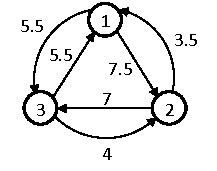
\includegraphics[scale=0.75]{Graficos/fig8_RB}		}{  \caption*{Grafo \(V\)}	}
	%
\end{floatrow}
\end{figure}


\begin{table}[H]
   \fontsize{7}{11}\selectfont
   	\captionsetup{justification=centering, labelfont=footnotesize, font=footnotesize}
    \centering
	\begin{tabular}{c|c} \thickline
    \hline
     Votante &  Preferencia \\ \hline
    \(V_1\) & \(A_1 \succ A_2 \sim A_3\)  \\
    \(V_2\) & \(A_1 \succ A_2 \succ A_3\)  \\
    \(V_3\) & \(A_1 \sim A_2 \succ A_3\)  \\
    \(V_4\) & \(A_1 \succ A_2 \succ A_3\)  \\
    \(V_5\) & \(A_1 \succ A_2 \succ A_3\)  \\
    \(V_6\) & \(A_2 \succ A_3 \succ A_1\)  \\
    \(V_7\) & \(A_2 \succ A_3 \succ A_1\)  \\
    \(V_8\) & \(A_3 \succ A_1 \succ A_2\)  \\
    \(V_9\) & \(A_1 \sim A_2 \sim A_3\)  \\
    \(V_{10}\) & \(A_3 \succ A_1 \succ A_2\)  \\
    \(V_{11}\) & \(A_3 \succ A_1 \sim A_2\)  
	\end{tabular}
\label{tab:B32} 
\end{table}
%
\end{ejem}

\vspace{-2\baselineskip}

\subsubsection{Regla de la Mayoría.}

En la regla de la mayoría, se elige a \(A_i\) como mejor alternativa a \(A_j\) ssi un mayor número de electores prefiere a \(A_i\) sobre \(A_j\) \cite{Dasgupta-2003}.\\


\begin{ejem} 
Para el ejemplo 14, las votaciones mayoritarias son: \(A_1 \succ A_2\): 7.5 votos a favor; \(A_2 \succ A_3\): 7 votos a favor; \(A_1 \succ A_3\) y \(A_3 \succ A_1\) 5.5 votos a favor de cada opción, empate. No hay un ganador. Se forman ciclos: \footnote{Un ciclo es una secuencia de proposiciones que inician y terminan con una misma alternativa. En el grafo asociado, un ciclo es un camino cerrado que inicia en un nodo y que regresa al mismo recorriendo el grafo en el sentido de los arcos.} \(A_1 \succ A_2 \succ A_3 \succ A_1\); \(A_1 \succ A_3 \succ A_1\). 

\begin{figure}[H]
\begin{floatrow}
	\fontsize{7}{11}\selectfont
	\captionsetup{justification=centering, labelfont=footnotesize, font=footnotesize}
	%	Tabla
	\capbtabbox{%
	 \begin{tabular}{c|ccc} \thickline
	 & \(A_1\) & \(A_2\) & \(A_3\)    \\ \hline
    \(A_1\) & 0 & 7.5 & 5.5  \\
	\(A_2\) & 0 & 0 & 7  \\
    \(A_3\) & 5.5 & 0 & 0  \\
	\end{tabular}
	}{	  \caption*{Voto mayoritario.}%
	}
	%	Figura
	\ffigbox{	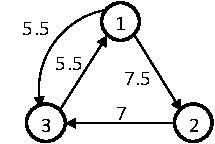
\includegraphics[scale=0.75]{Graficos/fig9_RB}		}{  \caption*{Grafo}	}
	%
\end{floatrow}
\end{figure}

\end{ejem}



\subsubsection{Método de Copeland.}

La matriz de pérdidas y ganancias \(R^* = (c_{ij})\) se define por \(c_{ij} = 1\) ssi \(\alpha_{ij} > \dfrac{n}{2}\), \(c_{ij} = -1\) ssi \(\alpha_{ij} < \dfrac{n}{2}\).
El puntaje de Copeland es igual a la suma de la fila de la matriz de pérdidas y ganancias \cite{Conitzer-2012, Levin-1995}. Las alternativas se ordenan en función del puntaje de Copeland. 

\begin{ejem} Para el ejemplo 14

\begin{table}[H]
   \fontsize{7}{11}\selectfont
   	\captionsetup{justification=centering, labelfont=footnotesize, font=footnotesize}
    \centering
	\begin{tabular}{c|ccccc} \thickline
    \hline
	 & \(A_1\) & \(A_2\) & \(A_3\) &  & \(C\)   \\ \hline
    \(A_1\) & 0 & 1 & 0 &  & 1 \\
	\(A_2\) & -1 & 0 & 1 &  & 0 \\
    \(A_3\) & 0 & -1 & 0 &  & -1 \\
	\end{tabular}
	\caption*{Matriz Copeland.}
\label{tab:B32} 
\end{table}

El orden agregado es: \(S_c: A_1 \succ A_2 \sim A_3\).

El método puede modificarse al método equivalente: La matriz de Copeland \(R^* = (c_{ij})\) se define por \(c_{ij} = 1\) ssi \(\alpha_{ij} \geq \dfrac{n}{2}\). El puntaje total de la alternativa \(A_i\) es igual a la suma de los elementos de la fila \(i\) menos la suma de los elementos de la columna \(i\) de la matriz \(R^*\). Las alternativas se ordenan en función del puntaje total.

\end{ejem}

\newpage
\begin{ejem} Continuando con el ejemplo 14:

\vspace{-1\baselineskip}
\begin{figure}[H]
\begin{floatrow}
	\fontsize{7}{11}\selectfont
	\captionsetup{justification=centering, labelfont=footnotesize, font=footnotesize}
	%	Tabla
	\capbtabbox{%
	 \begin{tabular}{c|ccccc} \thickline
	 & \(A_1\) & \(A_2\) & \(A_3\) &  & \(C\)   \\ \hline
    \(A_1\) & 0 & 1 & 1 &  & 1 \\
	\(A_2\) & 0 & 0 & 1 &  & 0 \\
    \(A_3\) & 1 & 0 & 0 &  & -1 \\
	\end{tabular}
	\vspace{0.5em}
	}{	  \caption*{Matriz de Copeland}%
	}
	%	Figura
	\ffigbox{	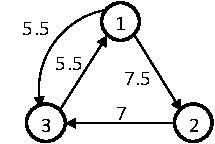
\includegraphics[scale=0.75]{Graficos/fig10_RB}		}{  \caption*{Grafo Copeland}	}
	%
\end{floatrow}
\end{figure}
\end{ejem}

%\vspace{-1\baselineskip}

La relación de Copeland es una forma de expresar la regla de la mayoría. En el grafo de la matriz de Copeland en estricto rigor no se ponderan los arcos; sin embargo, para presentar mayor información, y que quede claro su relación con la regla de la mayoría, se presenta la ponderación de los arcos.

\vspace{-0.5\baselineskip}

\subsubsection{Método de Condorcet.}

En el leguaje de Condorcet una <<proposición>> es la comparación de un par de alternativas (por ejemplo, \(A_3 \succ A_2\)) una <<opinión>> es un conjunto de proposiciones. La proposición inversa de \(A_i \succ A_j\) es \(A_j \succ A_i\). Una opinión es <<contradictoria>>, <<absurda>> o <<imposible>> si las proposiciones que la conforman generan un ciclo; una opinión es <<no contradictoria>> si no hay ciclos.

\vspace{1\baselineskip} 
El método de Condorcet consiste en: 
\begin{seriate}
\item Tomar las proposiciones que estén de acuerdo con el mayor número de votantes y analizar si dichas proposiciones no generan ciclos.
\item Si este es el caso, la opinión conformada por estas proposiciones es el orden que está de acuerdo con la mayoría de votantes.
\item Si hay ciclos, se toman las proposiciones que tengan menor votación y se las va borrando sucesivamente hasta eliminar los ciclos.
\item el orden final se construye a partir de las proposiciones remanentes (Young, 1990:28).
\end{seriate}

\vspace{1\baselineskip} 
El método de Condorcet en términos de grafo consiste en verificar si el grafo de la relación de Copeland es acíclico; si ese es el caso, se termina el proceso. Si no es así, hay que borrar los arcos de menor peso consecutivamente hasta obtener un grafo acíclico.

\begin{ejem} Para el ejemplo 14, el grafo de la relación de Copeland tiene ciclos. Al aplicar el método de Condorcet nos queda:

\vspace{-1\baselineskip}

\begin{center}
\begin{figure}[H]
	\fontsize{7}{11}\selectfont
	\captionsetup{justification=centering, labelfont=footnotesize, font=footnotesize}
    \centering
    \caption*{Relación de Copeland \(\qquad \qquad  R^* \backslash \{\text{arcos de menor peso}\} \qquad \qquad  \qquad  \mathcal{R}\)}
    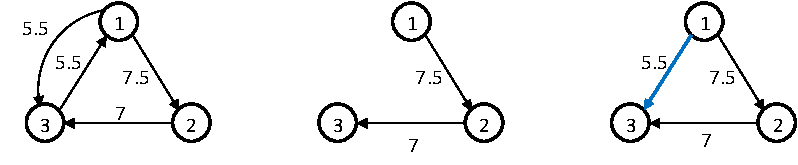
\includegraphics[scale=0.75]{Graficos/fig11_RB}	
    \label{fig:RB_grafo11}
\end{figure}
\end{center}

\end{ejem}

\subsubsection{Método de Borda.}
El método de Borda consiste en:

\begin{APAenumerate}
    \item De acuerdo al criterio de cada votante:
        \begin{seriate}
            \item Ordenar las alternativas descendentemente -de mejor a peor-.
            \item Asignar el valor \(n-1\) a la mejor alternativa, \(n-2\) a la siguiente mejor y así sucesivamente.
        \end{seriate}
    \item Calcular la cuenta o puntuación de Borda sumando los puntajes obtenidos.
    \item El orden resultante se define en función de la puntuación total \cite{Conitzer-2012, Levin-1995}. 
\end{APAenumerate}

El método puede ampliarse para cuando un elector establece empates entre las alternativas. En un primer paso, las alternativas que empatan se ordenan de manera arbitraria; en el segundo paso, el puntaje asignado a todas las alternativas empatadas es el promedio de los puntajes.


\begin{ejem} Para la votación del ejemplo 14, tenemos:

\begin{table}[H]
   \fontsize{7}{11}\selectfont
   	\captionsetup{justification=centering, labelfont=footnotesize, font=footnotesize}
    \centering
	\begin{tabular}{c|ccccccccccccc} \thickline
	 & \(C_1\) & \(C_2\) & \(C_3\) & \(C_4\)& \(C_5\)& \(C_6\)& \(C_7\)& \(C_8\)& \(C_9\)& \(C_10\)& \(C_11\)&  & \(B\)   \\ \hline
    \(A_1\) & 2 & 2 & 1.5 & 2 & 2 & 0 & 0 & 1 & 1 & 1 & 0.5 &  & 13 \\
	\(A_2\) & 0.5 & 1 & 1.5 & 1 & 1 & 2 & 2 & 0 & 1 & 0 & 0.5 &  & 10.5 \\
    \(A_3\) & 0.5 & 0 & 0 & 0 & 0 & 1 & 1 & 2 & 1 & 2 & 2 &  & 9.5 \\
	\end{tabular}
	\caption*{Cuenta de Borda}
\label{tab:B32} 
\end{table}

El método de Borda es equivalente a sumar los elementos de las filas de la matriz de votación:

\begin{table}[H]
   \fontsize{7}{11}\selectfont
   	\captionsetup{justification=centering, labelfont=footnotesize, font=footnotesize}
    \centering
	\begin{tabular}{c|ccccc} \thickline
	 & \(A_1\) & \(A_2\) & \(A_3\) &  & B   \\ \hline
    \(A_1\) & 0 & 7.5 & 5.5 &  & 13  \\
	\(A_2\) & 3.5 & 0 & 7 &  & 10.5 \\
    \(A_3\) & 5.5 & 4 & 0 &  & 9.5 \\
	\end{tabular}
\label{tab:B32} 
\end{table}

El orden agregado es: \(S_B : A_1 \succ A_2 \succ A_3\).

\end{ejem}

\subsubsection{Aplicación de los métodos de votación al análisis multicriterio.}

Para aplicar los métodos de votación al análisis multicriterio, primero se debe transformar cada <<criterio>> en un <<voto>>. Una posible forma de hacerlo es considerar un modelo con umbral.

\paragraph{Modelo con umbral.}

Sean \(x,y \in X = \Re ^n\) dos alternativas, \(c_j\) el umbral de indiferencia asociado al criterio \(x\). La preferencia parcial estricta y la indiferencia parcial se definen por:
\begin{equation*}
\left\{
\begin{aligned}
x \, P_j \, y & \Leftrightarrow x_j > y_j +c_j\\
x \, I_j \, y & \Leftrightarrow |x_j -y_j| \leq c_j
\end{aligned}
\right.
\end{equation*}



\newpage
\begin{ejem} Consideremos la siguiente matriz de impacto:

\begin{table}[H]
   \fontsize{7.5}{11}\selectfont
   	\captionsetup{justification=centering, labelfont=footnotesize, font=footnotesize}
    \centering
	\begin{tabular}{l|cccccc} \thickline
	 \multirow{2}{*}{Criterio} 	& \multirow{2}{*}{PIB pc} & \multirow{2}{*}{Inflación} & Consumo & Emisiones  & \multirow{2}{*}{Desempleo} & \multirow{2}{*}{Pobreza}	\\
	 		&		&		&	Energía pc &	 \(CO_2\) pc	 \\     \hline
    Objetivo & \(\max\) & \(\min\) & \(\min\) & \(\min\) & \(\min\) & \(\min\)   \\
	Umbral & 600 & 0.50 & 100 & 200 & 1.50 & 1.50 \\
    \cellcolor{pastelyellow} Ecuador & 7830 & 3.6 & 836.3 & 2111 & 5.0 & 5.48 \\
	\cellcolor{pastelyellow} Colombia & 9000 & 2.3 & 696.3 & 1560 & 11.6 & 9.64 \\
	\cellcolor{pastelyellow} Perú & 8790 & 1.5 & 667.1 & 1646 & 7.9 & 5.00 \\
	\end{tabular}
\label{tab:B32} 
\end{table}

Al aplicar la Definición 1, las relaciones entre las alternativas quedan:

\begin{table}[H]
   \fontsize{7}{11}\selectfont
   	\captionsetup{justification=centering, labelfont=footnotesize, font=footnotesize}
    \centering
	\begin{tabular}{l|c} \thickline
	Criterio & Preferencia  \\ \hline
    PIB pc & \(C \sim P \succ E\)   \\
	Inflación & \(P \succ C \succ E\)   \\
    Consumo Energía pc & \(C \sim P \succ E\)   \\
	Emisiones \(CO_2\) pc & \(C \sim P \succ E\)   \\
	Desempleo & \(E \succ P \succ C\)   \\
	Pobreza & \(P \sim E \succ C\)   \\
	\end{tabular}
\label{tab:B32} 
\end{table}

Que nos lleva a la matriz de <<votación>> siguiente:

\begin{figure}[H]
\centering
\begin{floatrow}
	\fontsize{7}{11}\selectfont
	\captionsetup{justification=centering, labelfont=footnotesize, font=footnotesize}
	%	Tabla
	\capbtabbox{%
	 \begin{tabular}{c|ccccc} \thickline
	 & ECU  & COL & PER & & B   \\ \hline
     ECU  & 0 & 2 & 1.5 & & 3.5   \\
	 COL  & 4 & 0 & 3 & & 7       \\
     PER  & 4.5 & 3 & 0 & & 7.5   \\
	\end{tabular}
	\vspace{1.1em}
	}{	  \caption*{Matriz de votación}%
	}
	%	Figura
	\ffigbox{	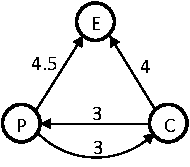
\includegraphics[scale=0.75]{Graficos/fig12_RB}		}{  \caption*{Grafo Copeland}	}
	%
\end{floatrow}
\end{figure}

\vspace{-1\baselineskip}
\[
	\text{Perú} \succ \text{Colombia} \succ \text{Ecuador}
\]

La aplicación del método de Condorcet lleva a soluciones múltiples una de las cuales coincide con el método de Borda:
\begin{align*}
	\text{Perú} \succ \text{Colombia} \succ \text{Ecuador}
\\
	\text{Colombia} \succ \text{Perú} \succ \text{Ecuador}
\end{align*}

\end{ejem}

\subsection{Axiomas de la elección social}

Es bien conocido que Kenneth Arrow dio un tratamiento axiomático a la Teoría de la Elección Social. Arrow primero estableció ciertas condiciones o propiedades (axiomas) razonables que se considera deben cumplir las reglas de agregación de las preferencias, para luego intentar encontrar la regla que satisfaga estos axiomas. Al final Arrow demostró que tal regla no existe \footnote{Erik Maskin (Maskin, 2009:6) al referirse Arrow comenta: Aunque la regla de la mayoría viola la decisión y la regla de la mayoría viola la independencia, Ken pensó que seguramente debe haber otras reglas de votación que satisfacen los cuatro axiomas: decidibilidad, consenso, ausencia de un dictador y la independencia de alternativas irrelevantes. Pero después de probar regla tras regla, con el tiempo llegó a sospechar que estos axiomas son colectivamente contradictorios. Y así es como nació el teorema de imposibilidad, Ken mostró que no hay una regla de votación que satisfaga los cuatro axiomas.}. Sin embargo, al aplicar cualquier método de agregación debería estar claro cuáles propiedades se satisfacen y cuáles no (de acuerdo a Arrow no es posible que se satisfagan todas). Veamos las propiedades de los operadores de agregación.

\vspace{1\baselineskip}
Sea \(\Re\) el conjunto de relaciones de preferencia racionales definidas sobre el conjunto de alternativas \(X = \{A_1,A_2,\dots, A_m\}\). Consideremos el operador \(\mathcal{H}\):
\begin{align*}
\mathcal{H}: \Re ^n & \rightarrow \Re \\
(R_1, R_2, \dots , R_n) & \mapsto R
\end{align*}


Sea \(\Omega = \{1,2,\dots, n\}\) el conjunto de índices de los individuos.

\vspace{1\baselineskip}
Para facilitar el enunciado a algunas de las propiedades veamos una definición previa.
Aumento del grado de preferencia. Se dice que el grado de la preferencia parcial entre \(A_i\) y \(A_j\) aumenta ssi de \(P_k^{-1}\) se pasa a \(I_k\) o \(P_k\), o de \(P_k\) se pasa a \(I_k\): \(P_k: (A_i \, P_k^{-1} \, A_j) \wedge [(A_i \, I'_k \, A_j) \vee (A_i \, P'_k \, A_j)]\) ó \((A_i \, I_k \, A_j) \wedge (A_i \, P'_k \, A_j)\). Para la preferencia agregada el grado de la preferencia entre \(A_i\) y \(A_j\) aumenta ssi de \(P^{-1}\) se pasa a \(I,J\) o \(P\); o de \(J\) se pasa a \(I\) O \(P\); de \(I\) se pasa a \(P\): \((A_i \, P^{-1} \, A_j) \wedge [(A_i \, I' \, A_j) \vee (A_i \, J' \, A_j) \vee (A_i \, P' \, A_j)]\) ó \((A_i \, J \, A_j) \wedge [(A_i \, I' \, A_j) \vee (A_i \, P' \, A_j)]\) ó \((A_i \, I \, A_j) \wedge (A_i \, P' \, A_j)\).

\subsubsection{Propiedades de los operadores.}

Se dice que el operador de agregación de preferencias \(\mathcal{H}\) es:

\begin{APAenumerate}
    \item \textbf{Paretiano:} ssi \(\mathcal{H}\) respeta la unanimidad de la preferencia estricta entre las alternativas. O sea, ssi para todos los individuos, la alternativa \(A_i\) es estrictamente preferida a \(A_j\), en la preferencia agregada también; es decir: \(\forall k \in \Omega, A_i \, P_k \, A_j \Rightarrow A_i \, P \, A_j\).
    
   \vspace{1\baselineskip}
    \item \textbf{Fuertemente Paretiano:} ssi para todos los individuos, la alternativa \(A_i\) es débilmente preferida a \(A_j\), y si para algún individuo es estrictamente preferida, en la preferencia agregada también lo es: \(\forall k \in \Omega, A_i \, R_k \, A_j \wedge \exists j \in \Omega,  A_i \, P_j \, A_j \Rightarrow A_i \, P \, A_j\).
    
    \vspace{1\baselineskip}
    \item \textbf{Simétrico entre criterios:} (anónimo) ssi no importa los nombres de los individuos. Es decir, hay un trato igualitario para todos ellos. Esto se estable de la manera siguiente: un cambio de orden entre los criterios no afecta el resultado del funcional. Si \(\sigma\) es una permutación de \(\Omega\), entonces:
    \[
    	\mathcal{H}(R_1, R_2, \dots, R_n) = \mathcal{H}(R_{\sigma (1)}, R_{\sigma (2)}, \dots, R_{\sigma (n)})
    \]
    
    \vspace{1\baselineskip}
    \item \textbf{Neutral entre alternativas:} ssi la preferencia agregada se invierte cuando se invierten las preferencias parciales originales.
    \[
    	\mathcal{H}(R_1^{-1}, R_2^{-1}, \dots, R_n^{-1}) = \mathcal{H}(R_{11}, R_{2}, \dots, R_{n})^{-1}
    \]
    
    \vspace{1\baselineskip}
    \item \textbf{Tiene respuesta positiva:} ssi en la preferencia agregada \(A_i\) es débilmente preferida a \(A_j\) y si aumenta el grado de preferencia parcial \(A_i\) sobre \(A_j\) para algún \(k \in \Omega\), entonces \(A_i\) es estrictamente preferido a \(A_j\). Si \(A_i \, R \, A_j\) y para algún \(k \in \Omega\), \(\{( A_i \, P_k^{-1} \, A_j) \wedge [( A_i \, I'_k \, A_j) \vee ( A_i \, P'_k \, A_j)]\} \vee \{( A_i \, I_k \, A_j) \wedge ( A_i \, P'_k \, A_j)\}\) entonces \(A_i \, P' \, A_j\); donde
\begin{align*}
	R &= \mathcal{H}(R_1, \dots, R_k, \dots, R_n) ,
	\\
	R' &= \mathcal{H}(R_1, \dots, R'_k, \dots, R_n).
\end{align*}
    
    Adicionalmente puede añadirse un axioma adicional relacionado con el axioma de respuesta positiva. 
    
        \begin{APAitemize}
            \item \textbf{No decreciente:} ssi el grado de la preferencia agregada entre \(A_i\) y \(A_j\) no decrece cuando aumenta el grado de preferencia de \(A_i\) sobre \(A_j\) para algún \(k \in \Omega\). Si para algún \(k \in \Omega\), \(\{(A_i \, P_k^{-1} \, A_j) \wedge [(A_i \, I'_k \, A_j) \vee (A_i \, P'_k \, A_j)]\} \vee \{(A_i \, I_k \, A_j) \wedge (A_i \, P'_k \, A_j)\}\)  entonces \((A_i \, I \, A_j) \Rightarrow [(A_i \, I' \, A_j) \vee (A_i \, P' \, A_j)] \vee (A_i \, J \, A_j) \Rightarrow [(A_i \, J' \, A_j) \vee (A_i \, P' \, A_j)] \vee (A_i \, P \, A_j) \Rightarrow (A_i \, P' \, A_j)\); donde \(R = \mathcal{H}(R_1, \dots, R_k, \dots, R_n) \), \(R' = \mathcal{H}(R_1, \dots, R'_k, \dots, R_n)\).
        \end{APAitemize}
    
    \vspace{1\baselineskip}
    \item \textbf{Satisface el axioma de independencia de alternativas irrelevantes:} ssi la relación agregada \(A_i \, R \, A_j\) depende únicamente de las preferencias entre estas alternativas. De manera formal, \(R_k\) y \(R'_k\) son relaciones en \(X\), \(k \in \Omega\), y si \(R_k : \{A_i, A_j\} = R'_k : \{A_i, A_j\}\) para todo \(k \in \Omega\), entonces: \((R_1, R_2, \dots, R_n) : \{A_i, A_j\}  = \mathcal{H}(R'_1,  R'_2, \dots, R'_n) : \{A_i, A_j\} \). \(R : Y\) es la restricción de la relación \(R\) al subconjunto de alternativas \(Y\).
    
    \vspace{1\baselineskip}
    \item \textbf{Dictatorial:} ssi existe un individuo \(k\) llamado dictador tal que la preferencia estricta del dictador determina la preferencia estricta agregada: \(A_i \, P_k \, A_j \Rightarrow A_i \, P \, A_j\).
    
    
    La definición de \(\mathcal{H}\) implícitamente define cuatro condiciones adicionales:
    
    \vspace{1\baselineskip}
    \item \textbf{Universalidad del dominio:} La regla de agregación \(\mathcal{H}\) se aplica a cualquier vector de preferencias racionales \((R_1, R_2, \dots, R_n).\)
    
    \vspace{1\baselineskip}
    \item \textbf{Racionalidad de la relación agregada:} La relación agregada \(R\) es completa, reflexiva y transitiva sobre el conjunto de alternativas \(X\) (es un orden o preorden total o completo).
    
    \vspace{1\baselineskip}
    \item \textbf{Decidibilidad débil:} En cualquier conjunto de alternativas \(X\) puede identificar un elemento máximo.
    
    \vspace{1\baselineskip}
    \item \textbf{Decidibilidad fuerte:} En cualquier conjunto de alternativas \(X\) puede identificar un único elemento máximo.
\end{APAenumerate}

\vspace{1\baselineskip}
\textbf{Observación.} La condición de simetría entre criterios es más general que la condición de no existencia de un dictador. De igual manera, si la relación agregada es un orden o preorden total, se cumple que es decidible fuerte o débil respectivamente.


Como un ejercicio para el lector queda propuesto verificar el cumplimiento de las propiedades de los operadores de agregación de los métodos de votación que se ha mencionado en este documento.
\newpage

\nocite{Burbano-2014, Burbano-2016, Burbano-2009, Cioni-2010, Colell-1995, Reina-2008}

}







\end{document}































